\documentclass[xcolor=table]{beamer}

\usetheme{Madrid} % Other popular themes: default, Madrid, Boadilla, AnnArbor, CambridgeUS
\usecolortheme{default}
\usefonttheme[onlymath]{serif}

% Custom colors for premium dark theme title slide
\definecolor{darkblue}{RGB}{15, 23, 42}
\definecolor{accentblue}{RGB}{56, 189, 248}
\definecolor{gold}{RGB}{245, 158, 11}

% Global color theme overrides for modern design system
\definecolor{primary}{RGB}{15, 23, 42}       % slate 900
\definecolor{secondary}{RGB}{71, 85, 105}    % slate 600
\definecolor{accent}{RGB}{2, 132, 199}       % sky 600

\setbeamercolor{structure}{fg=primary}
\setbeamercolor{palette primary}{bg=primary, fg=white}
\setbeamercolor{palette secondary}{bg=secondary, fg=white}
\setbeamercolor{palette tertiary}{bg=accent, fg=white}
\setbeamercolor{titlelike}{fg=white}

% Clean card blocks instead of heavy defaults
\setbeamercolor{block title}{bg=primary!10, fg=primary}
\setbeamercolor{block body}{bg=primary!5, fg=black}
\setbeamercolor{block title alerted}{bg=red!10, fg=red!70!black}
\setbeamercolor{block body alerted}{bg=red!5, fg=black}
\setbeamercolor{block title example}{bg=green!10, fg=green!50!black}
\setbeamercolor{block body example}{bg=green!5, fg=black}

% Clean modern circular itemize markers
\setbeamertemplate{items}[circle]
\setbeamercolor{item}{fg=accent}

% Hide navigation symbols
\setbeamertemplate{navigation symbols}{}
\setbeamertemplate{caption}[numbered]

% Title page details: 
\title[Modeling 2D Marshak Waves]{Modeling 2D Marshak Waves}
\subtitle{Understanding the physics of X-ray radiation-driven supersonic nonlinear heat waves}
\author[Kochavi et al.]{\textbf{Yuval Kochavi}, Tal Ramot, Tal Balakirski, Shay I. Heizler}
\date{June 17, 2026}

\begin{document}

% Title slide
{
\setbeamercolor{background canvas}{bg=darkblue}
\begin{frame}[plain]
    \centering
    {\Huge\bfseries\color{white} Modeling 2D \\ Marshak Waves}
    
    \vspace{0.4cm}
    {\small\color{white} Understanding the physics of X-ray radiation-driven supersonic nonlinear heat waves}
    
    \vspace{0.8cm}
    {\large \textbf{\color{white}Yuval Kochavi}}
    
    % \vspace{0.3cm}
    % {\small Racah Institute of Physics, \\ The Hebrew University of Jerusalem, Israel}
    
    \vspace{1.2cm}
    {\large\textbf{\color{white}Thesis presentation}}
\end{frame}
}

% Table of Contents
\begin{frame}{Outline}
    \tableofcontents
\end{frame}

\begin{frame}{About Me}
    \begin{itemize}
        \item 19 years old, from Petah Tikva.
        \item Studied Physics and Engineering at Bar-Ilan University during high school.
        \item Started research in semester C, after taking courses in Physics, Mathematics, and Computer Science in previous semesters.
    \end{itemize}
\end{frame}

% --- Section 1 ---
\section{Marshak Waves Experimental Setup}

\begin{frame}{Marshak Waves Experiments}
    Using a Hohlraum as an X-ray generator, a supersonic heat wave propagates in the low-density foam.
    
    \vspace{0.5cm}
    \begin{columns}
        \begin{column}{0.45\textwidth}
            \centering
            % \includegraphics[width=\textwidth]{figures/laser_pulse_graph.png}
            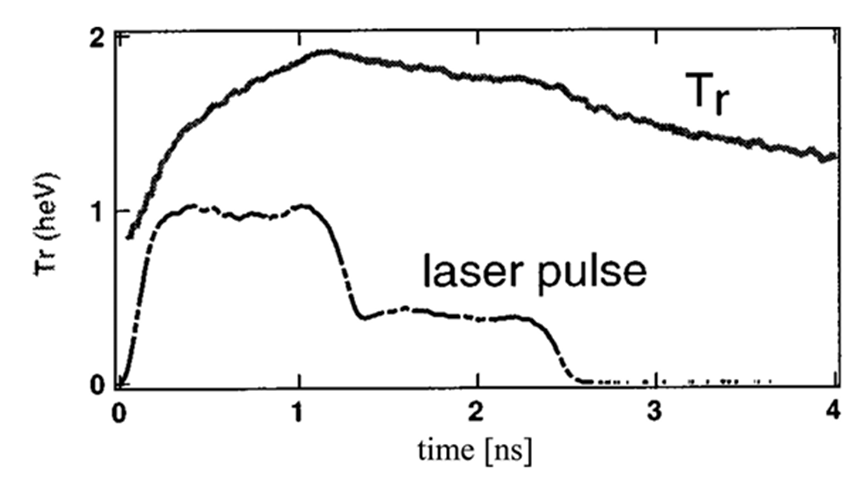
\includegraphics[width=\textwidth]{figures_intreduction/T_drive.png}

            {\scriptsize \textit{Back et al. POP, (2000)}}
        \end{column}
        \begin{column}{0.45\textwidth}
            \centering
            % \includegraphics[width=\textwidth]{figures/hohlraum_diagram.png}
            
\includegraphics[width=\textwidth]{figures_intreduction/setup.png}

            {\scriptsize \textit{Cohen et al. PRR, (2020)}}
        \end{column}
    \end{columns}

    \vspace{0.3cm}

    Laser $\Rightarrow$ Hohlraum $\Rightarrow$ X-ray radiation $\Rightarrow$ supersonic heat wave propagating in the low-density foam.
\end{frame}

\begin{frame}{Marshak Waves Experimental Setup}
    \begin{columns}
        \begin{column}{0.4\textwidth}
            \centering
            % \includegraphics[width=0.65\textwidth]{figures/radiograph.png} \\
            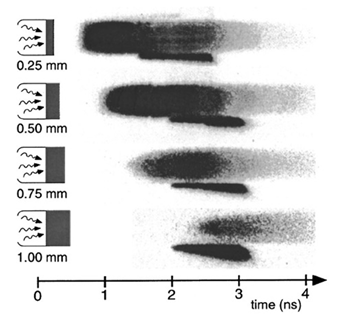
\includegraphics[width=0.56\textwidth]{figures_intreduction/method1.png} \\ % Placeholder

            {\scriptsize \textit{Back et al. POP, (2000)}}
            \vspace{0.1cm}
            % \includegraphics[width=0.65\textwidth]{figures/time_series.png} \\
            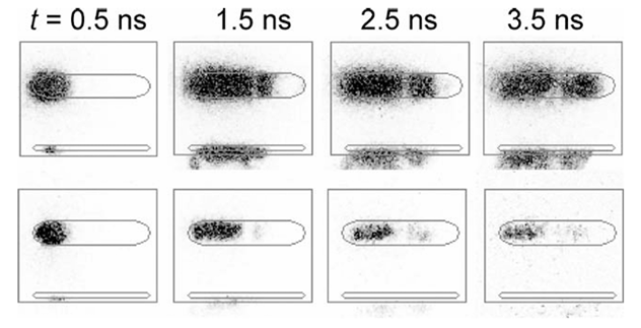
\includegraphics[width=0.56\textwidth]{figures_intreduction/method2.png} \\ % Placeholder

            {\scriptsize \textit{Rosen et al. ASS, (2006)}}
            \vspace{0.1cm}
            % \includegraphics[width=0.65\textwidth]{figures/foam_tube.png}
            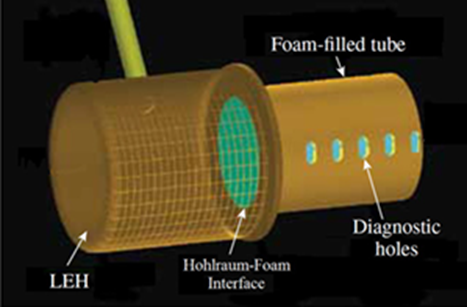
\includegraphics[width=0.56\textwidth]{figures_intreduction/method3.png}    % Placeholder

            {\scriptsize \textit{Cohen et al. PRR, (2020)}}
        \end{column}
        
        \begin{column}{0.1\textwidth}
            \centering
            \Huge $\Rightarrow$ \\
            \vspace{1.5cm}
            \Huge $\Rightarrow$
        \end{column}
        
        \begin{column}{0.5\textwidth}
            There are several ways to track the heat wave propagation in experiments:

            
            \centering
            % \includegraphics[width=0.8\textwidth]{figures/ta2o5_top_graph.png} \\
            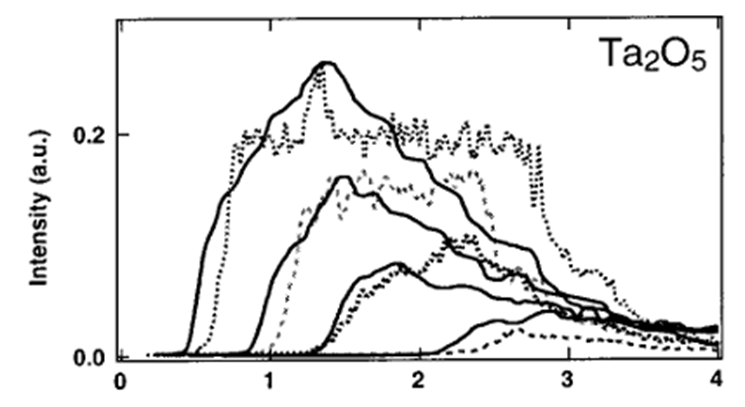
\includegraphics[width=0.9\textwidth]{figures_intreduction/flux.png} \\ % Placeholder

            {\scriptsize \textit{Back et al. POP, (2000)}}
            \vspace{0.2cm}
            % \includegraphics[width=0.8\textwidth]{figures/ta2o5_bottom_graph.png}
            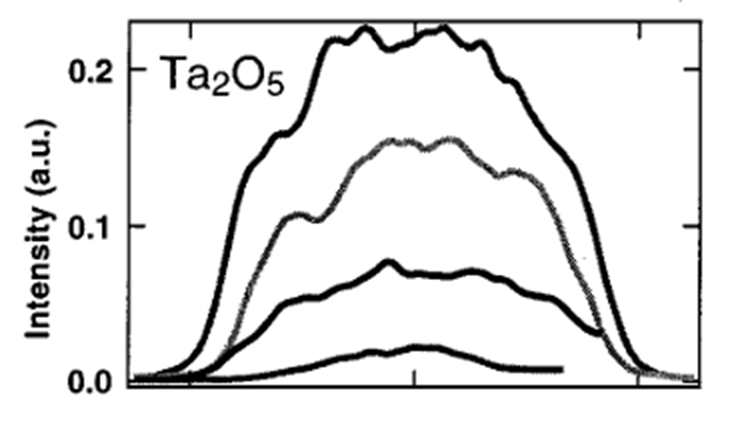
\includegraphics[width=0.9\textwidth]{figures_intreduction/flux_curvature.png}

            {\scriptsize \textit{Back et al. POP, (2000)}}
        \end{column}
    \end{columns}
\end{frame}

\begin{frame}{Experiments Tested}
    \begin{table}
        \centering
        \small
        \renewcommand{\arraystretch}{1.1}
        \rowcolors{2}{primary!5}{white}
        \begin{tabular}{llcc}
            \hline \hline
             & & density & temperature \\
            The experiment & foam type & (mg/cc) & (eV) \\
            \hline
            Massen \textit{et al.} & $\mathrm{C}_{11}\mathrm{H}_{16}\mathrm{Pb}_{0.3852}$ & 80 & 100--150 \\
            Back \textit{et al.} & $\mathrm{SiO}_2$, $\mathrm{Ta}_2\mathrm{O}_5$ & 10--50 & 85--190 \\
            Xu \textit{et al.} & \begin{tabular}{@{}l@{}}$\mathrm{C}_6\mathrm{H}_{12}$, \\ $\mathrm{C}_6\mathrm{H}_{12}\mathrm{Cu}_{0.394}$\end{tabular} & 50 & 160 \\
            Ji-Yan \textit{et al.} & $\mathrm{C}_8\mathrm{H}_8$ & 160 & 175 \\
            Keiter \textit{et al.} & \begin{tabular}{@{}l@{}}$\mathrm{C}_{15}\mathrm{H}_{20}\mathrm{O}_6$, \\ $\mathrm{C}_{15}\mathrm{H}_{20}\mathrm{O}_6\mathrm{Au}_{0.172}$\end{tabular} & 45--70 & 200--210 \\
            Moore \textit{et al.} & $\mathrm{SiO}_2$, $\mathrm{C}_8\mathrm{H}_7\mathrm{Cl}$ & 90--120 & 310 \\
            Courtois \textit{et al.} & $\mathrm{SiO}_2$ & 19 -- 29 & 170 \\
            \hline \hline
        \end{tabular}
    \end{table}
\end{frame}

\section{Describing the System}

\begin{frame}{The Governing Equations}
    Scattering-free gray Boltzmann equation for photons (RTE):
    \begin{multline}
        \frac{1}{c}\frac{\partial I(\hat{\Omega},\vec{r},t)}{\partial t}+\hat{\Omega}\cdot \vec{\nabla}I(\hat{\Omega},\vec{r},t)=
        \sigma'_{a}(T_m)\left(B(T_m(\vec{r},t))-I(\hat{\Omega},\vec{r},t)\right)
    \end{multline}
    
    \vspace{0.5cm}
    Energy exchange between radiation and matter:
    \begin{equation}
        \frac{C_v(T_m)}{c} \frac{\partial T_m}{\partial t} = \sigma_a'(T_m) \left( \frac{1}{c} \int_{4\pi} I \, d\hat{\Omega} - aT_m^4 \right)
    \end{equation}
\end{frame}

\begin{frame}{From RTE to Moment Equations}
    We can define the energy density and flux:
    \begin{equation*}
        E(\vec{r},t) = \frac{1}{c}\int_{4\pi} I(\hat{\Omega}, \vec{r}, t) \, d\hat{\Omega}, \qquad \vec{F}(\vec{r},t) = \int_{4\pi} I(\hat{\Omega}, \vec{r}, t)\hat{\Omega} \, d\hat{\Omega}
    \end{equation*}

    Now the Boltzmann equation takes the following form:
    \begin{gather*}
        \frac{\partial E(\vec{r},t)}{\partial t} + \nabla \cdot \vec{F}(\vec{r},t) = \sigma_a'(T_m)\left(\int_{4\pi} \frac{B(\vec{r},t)}{c} \, d\hat{\Omega} - E(\vec{r},t)\right) \\[8pt]
        \frac{1}{c}\frac{\partial \vec{F}(\vec{r},t)}{\partial t} + \frac{c}{3} \nabla E(\vec{r},t) + \sigma_a'(T_m)\vec{F}(\vec{r},t) = 0
    \end{gather*}
\end{frame}

\begin{frame}{The Diffusion Approximation}
    Assuming the change of the flux in time is small ($\frac{1}{c}\frac{\partial \vec{F}}{\partial t} \approx 0$):
    \begin{equation*}
        \vec{F}(\vec{r},t) = -\frac{c}{3\sigma_a'(T_m)} \nabla E(\vec{r},t)
    \end{equation*}

    \vspace{0.3cm}
    This turns Boltzmann into the diffusion equation:
    \begin{equation*}
        \frac{\partial E(\vec{r},t)}{\partial t} - \nabla \cdot \left[\overbrace{\frac{c}{3\sigma_t(T_m)}}^{D(T_m)} \nabla E(\vec{r},t)\right] = c\sigma_a'(T_m)\left(\overbrace{\int_{4\pi} \frac{B(\vec{r},t)}{c} \, d\hat{\Omega}}^{U_R(\vec{r},t)} - E(\vec{r},t)\right)
    \end{equation*}
\end{frame}

\begin{frame}{Gray Coupled Equations and LTE}
    From the diffusion equation, setting $\int_{4\pi} \frac{B}{c}\,d\hat{\Omega} = aT_m^4$, the coupled gray radiation-matter system reads,
    \begin{align*}
        \frac{\partial E}{\partial t} - \nabla \cdot \left(\frac{c}{3\sigma} \nabla E\right) &= c\sigma(aT_m^4 - E), \quad \quad \quad E = \mathrm{a} T_R^4 \\
        \rho \frac{\partial e}{\partial t} &= c\sigma(E - aT_m^4)
    \end{align*}

    Finally, assuming thermodynamic equilibrium (TE) between the radiation field and the material ($T \equiv T_R = T_m$):
    \begin{equation}
        \frac{\partial T^4}{\partial t} + \rho \frac{\partial e}{\partial t} = \nabla \cdot \left(\frac{c}{3\sigma} \nabla (aT^4)\right)
    \end{equation}

\end{frame}

\begin{frame}{The Problem}
    \begin{columns}
        \begin{column}{0.58\textwidth}
            \begin{itemize}
                \item Power-law approximation for specific energy and opacity:
                \begin{equation*}
                    e = fT^\beta \rho^{-\mu}, \qquad \frac{1}{\sigma} = \frac{1}{\rho \kappa} = gT^\alpha \rho^{-\lambda - 1}
                \end{equation*}
            \end{itemize}
            
            \vspace{-0.2cm}
            \begin{alertblock}{The Core Challenge}
                The diffusion coefficient $D=\frac{c}{3\rho \kappa}$ and the material internal energy $e$ are highly nonlinear. The system becomes very difficult to solve analytically.
            \end{alertblock}
            
        \end{column}
        \hfill
        \begin{column}{0.38\textwidth}

            \centering
            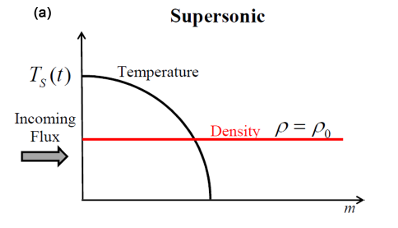
\includegraphics[width=\textwidth]{figures_intreduction/supersonic.png}
            
            \vspace{0.2cm}
            {\scriptsize \textit{Shussman et al. POP, (2015)}}
        \end{column}
    \end{columns}
\end{frame}

\begin{frame}{The Goal}
    \begin{block}{Goal}
       Build a 2D semi-analytical model to understand supersonic heat wave propagation and temperature distribution.
    \end{block}

    \begin{columns}
        \begin{column}{0.5\textwidth}

            \vspace{0.2cm}
            Specifically, analyzing the following equation:

            \begin{equation*}
                \frac{\partial T^4}{\partial t} + f \rho^{-\mu+1}\frac{\partial T^{\beta}}{\partial t} = \nabla \cdot \left(D(T)\nabla (aT^4)\right)
            \end{equation*}

            using cylindrical coordinates and the relevant boundary conditions.
                    
        \end{column}
        \hfill
        \begin{column}{0.48\textwidth}

            \centering
            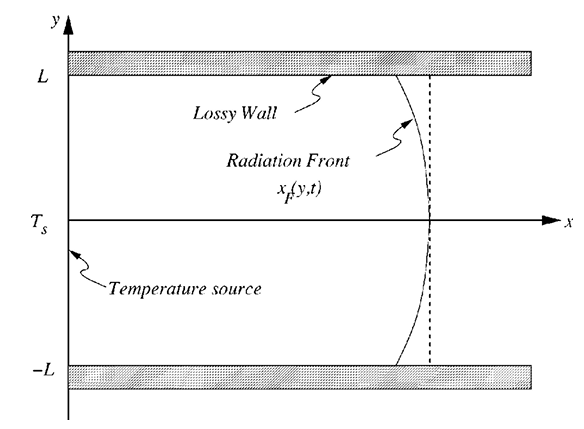
\includegraphics[height=0.5\textheight]{figures_intreduction/hurricane.png}
        \end{column}
    \end{columns}
\end{frame}

% --- Section 3 ---
\section{1.5D Model}

{
\setbeamercolor{background canvas}{bg=darkblue}
\begin{frame}[plain]
    \vfill
    \begin{center}
        {\Huge\bfseries\color{white} 1.5D Model}
    \end{center}
    \vfill
\end{frame}
}

\begin{frame}{HR Model - Governing Equations}
    Hammer and Rosen solved the diffusion equation with the specific energy and opacity power laws:
    \begin{equation*}
        e = fT^\beta \rho^{-\mu}, \qquad \frac{1}{\kappa} = gT^\alpha \rho^{-\lambda}
    \end{equation*}
    where $f, \mu, g, \lambda, \alpha, \beta$ are material-dependent parameters.

    Assuming $\rho f T^\beta \rho^{-\mu + 1} \gg aT^4$ (true up to $\sim$3~keV), HR solved:
    \begin{align*}
        f \rho^{-\mu + 1}\frac{\partial T^{\beta}}{\partial t} = \frac{\partial}{\partial x} \cdot \left(\frac{c g T^\alpha \rho^{-\lambda - 1}}{3} \frac{\partial}{\partial x} (aT^4)\right)
    \end{align*}
    
    Using perturbation theory, HR derived key physical quantities.
    \vfill
    \begin{flushright}
        {\scriptsize \textit{Rosen et al. POP, (2003)}}
    \end{flushright}
\end{frame}

\begin{frame}{HR Model - Heat Front Solution}
    The heat front position $x_F(t)$ is given by:
    \begin{equation*}
        \boldsymbol{x_F^2(t) = \frac{2 + \varepsilon}{1 - \varepsilon} C H^{-\varepsilon}(t) \int_0^t H(t') \, dt'}
    \end{equation*}
    
    where:
    \begin{equation*}
        C = \frac{16g\sigma_{SB}}{3f(4+\alpha)} \rho^{2-\mu-\lambda}; \quad \varepsilon = \frac{\beta}{4+\alpha}
    \end{equation*}
    \begin{equation*}
        H(t) = T_s^{4+\alpha}(t)
    \end{equation*}
    where $T_s$ is the \textbf{surface temperature} at $x=0$.

\end{frame}

\begin{frame}{HR 1D Model Limitations}
    Naive HR misses the experimental results of Back et al. by a factor of 2!
    
    \vspace{0.1cm}
    \begin{figure}
        \centering
        
\includegraphics[width=0.68\textwidth]{figures_1.5model/HR.png}
    \end{figure}

    \textbf{Conclusion}: Assuming $T_s = T_D$ overestimates the wave speed.
\end{frame}

\subsection{1D Effects}
\begin{frame}{Marshak Boundary Condition: $T_D \neq T_s$}
    The Marshak boundary condition states that
    \begin{equation*}
        \sigma_{SB} T_D^4(t) = \int_0^1 I(\mu)\mu d\mu = \frac{cE(0,t)}{4} + \frac{F(0,t)}{2}
    \end{equation*}
    where $F(0,t)$ is the net flux entering the foam. 
    
    This leads to:
    \begin{equation*}
        \sigma_{SB} T_D^4(t) = \sigma_{SB} T_s^4(t) + \frac{F(0,t)}{2}
    \end{equation*}
    Therefore, the surface temperature $T_s$ is \textbf{always lower} than the drive temperature $T_D$!
\end{frame}

\begin{frame}{Marshak Boundary Condition: $T_D \neq T_s$}
    Applying the Marshak boundary condition slows the propagation front significantly:
    
    \vspace{0.2cm}
    \begin{figure}
        \centering
        
\includegraphics[width=0.7\textwidth]{figures_1.5model/marshak.png}
    \end{figure}
\end{frame}

\subsection{2D Effects}
{
\setbeamercolor{background canvas}{bg=darkblue}
\begin{frame}[plain]
    \vfill
    \begin{center}
        {\color{accentblue}\LARGE 1.5D Model} \\
        \vspace{0.4cm}
        {\huge\bfseries\color{white} 2D Effects}
    \end{center}
    \vfill
\end{frame}
}

\begin{frame}{Energy Wall Loss - Gold}
    The heat wave in the foam loses energy to the gold walls, which slows it down:
    \begin{itemize}
        \item Subsonic energy loss of gold per unit area:
        \begin{equation*}
            E_{\mathrm{gold}}(t) = 0.59\, T_s^{3.35}\, [t - t_0(x)]^{0.59} \quad [\mathrm{hJ/mm^2}]
        \end{equation*}
        where $t_0(x)$ is the front arrival time at position $x$.
        \item Energy loss from a tube segment of length $dx$:
        \begin{equation*}
            dE_W = E_{\mathrm{gold}}(t - t_0(x)) \cdot 2\pi R \, dx
        \end{equation*}
        \item Total accumulated energy loss in the wall up to time $t$:
        \begin{equation*}
            E_W(t) = 2\pi R \int_0^{x_F(t)} \int_{t_0(x)}^t \dot{E}_{\mathrm{gold}}(t') \, dt' \, dx
        \end{equation*}
    \end{itemize}
    
    \begin{alertblock}{2D Effect Integration}
        This energy is subtracted from the foam's energy at each iteration, thereby introducing a two-dimensional effect.
    \end{alertblock}
\end{frame}

\begin{frame}{Modeling Other Wall Materials}
    The same 2D wall loss framework can be applied to other wall materials by using their respective energy loss fits:
    \begin{itemize}
        \item \textbf{Copper (Cu) - Mid-Z (subsonic fit): }
        \begin{equation*}
            E_{\mathrm{copper}}(t) = 1.58\, T_s^{3.40}\, [t - t_0(x)]^{0.61} \quad [\mathrm{hJ/mm^2}]
        \end{equation*}
        \item \textbf{Beryllium (Be) - Low-Z (supersonic fit):}
        \begin{equation*}
            E_{\mathrm{be}}(t) = 1.27\, T_s^{4.99}\, [t - t_0(x)]^{0.50} \quad [\mathrm{hJ/mm^2}]
        \end{equation*}
        \item \textbf{Vacuum (no external material):}
        \begin{equation*}
            dE_{\mathrm{vacuum}} = \sigma_{\mathrm{SB}} T_s^4 \, dt \quad (\text{No re-emission from walls})
        \end{equation*}
    \end{itemize}
\end{frame}

\begin{frame}{Effect of Wall Loss}
    Including wall loss reduces the front velocity:
    
    \vspace{0.2cm}
    \begin{figure}
        \centering
        
\includegraphics[width=0.7\textwidth]{figures_1.5model/wall_loss.png}
    \end{figure}
\end{frame}

\begin{frame}{Wall Ablation - Changing Foam Radius}
    Gold wall material absorbs energy and ablates inward:
    \begin{columns}
        \begin{column}{0.54\textwidth}
            \begin{itemize}
                \item Inward wall velocity:
                \begin{equation*}
                    u_{\mathrm{abl}} = -510.1\,\tilde{u}\,T_s^{0.716}\,[t - t_0(x)]^{0.036}
                \end{equation*}
                \item Shrunk cylinder radius:
                \begin{equation*}
                    R(t,x) = R_0 - u_{\mathrm{abl}}(x,t)(t - t_0(x))
                \end{equation*}
                \item Reduced inlet energy:
                \begin{equation*}
                    E_{\mathrm{in}}(t) = 2\pi\sigma_{\mathrm{SB}} \int_0^t R^2(t',0) \left[ T_D^4(t') - T_s^4(t') \right] dt'
                \end{equation*}
            \end{itemize}
        \end{column}
        \hfill
        \begin{column}{0.42\textwidth}
            \centering
            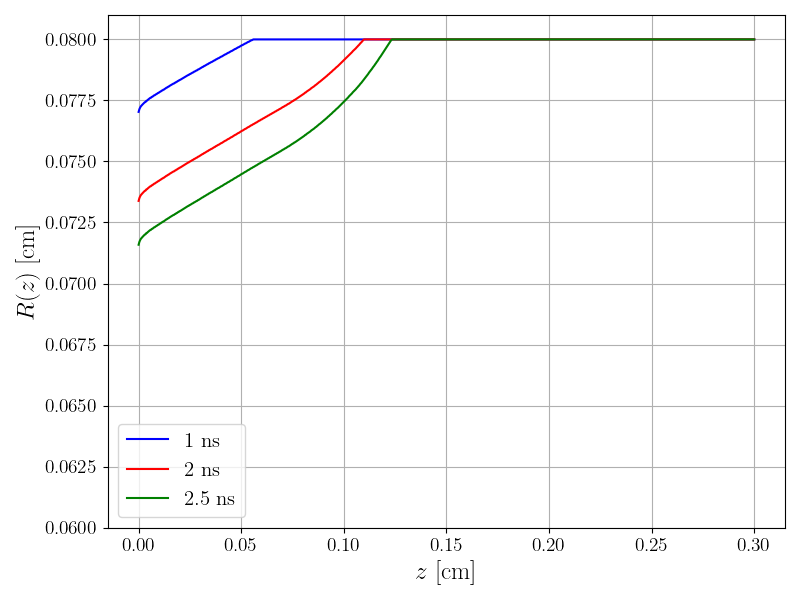
\includegraphics[width=\textwidth]{figures_1.5model/radius_ablation.png}
        \end{column}
    \end{columns}
\end{frame}

\begin{frame}{Wall Ablation - Changing Foam Density}
    The ablated wall material compresses and densifies the adjacent foam:
    \begin{columns}
        \begin{column}{0.54\textwidth}
            \begin{itemize}
                \item Mass conservation:
                \begin{equation*}
                    \rho_{\mathrm{eff}}(t) = \rho_0 \frac{V_0}{V(t)}
                \end{equation*}
                \item Effective density:
                \begin{equation*}
                    \rho_{\mathrm{eff}}(t) = \frac{\rho_0 V_0}{\int_0^{x_F(t)} \pi R^2(t,x) \, dx}
                \end{equation*}
            \end{itemize}
        \end{column}
        \hfill
        \begin{column}{0.42\textwidth}
            \centering
            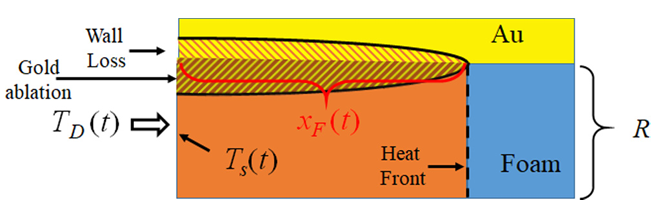
\includegraphics[width=\textwidth]{figures_1.5model/ablation.png}
        \end{column}
    \end{columns}
\end{frame}


\begin{frame}{Effect of Wall Ablation}
    Inward wall ablation compressively densifies the foam, slowing down propagation significantly:
    
    \vspace{0.2cm}
    \begin{figure}
        \centering
        
\includegraphics[width=0.7\textwidth]{figures_1.5model/denser_foam.png}
    \end{figure}
\end{frame}

\begin{frame}{Effective Mean Free Path}
    When $\lambda_R \ge 2R$, wall collisions control the transport instead of diffusion.

    This can be modeled as (\textit{Courtois et al. POP, (2024)}):
    \begin{equation*}
        \frac{1}{\lambda_{\mathrm{eff}}} = \frac{1}{\lambda_R} + \frac{1}{2R}, \quad \quad \text{$\lambda_R$ is the Rosseland mean free path}
    \end{equation*}
    
    A smoother transition is defined using the generalized power mean:
    \begin{equation*}
        \lambda_{\mathrm{eff}} = \left( (2R)^{-n} + \lambda_{\mathrm{R}}^{-n} \right)^{-1/n}
    \end{equation*}

    \begin{columns}
        \begin{column}{0.45\textwidth}
            \centering
            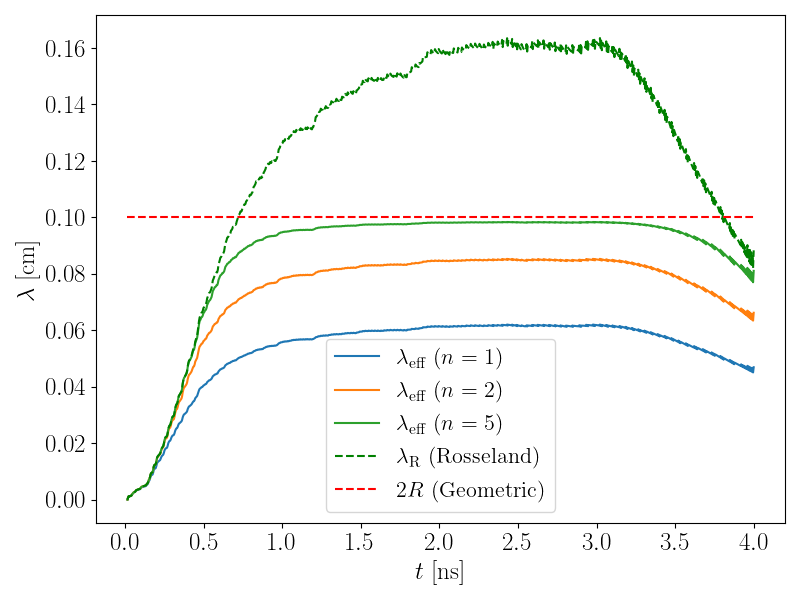
\includegraphics[width=0.95\textwidth]{figures_1.5model/lam_eff0.png}
            \raisebox{3.2cm}[0pt][0pt]{\makebox[0pt][l]{\hspace{-0.84\textwidth}\fcolorbox{blue!40}{white}{\strut\scriptsize\textbf{SiO$_2$}}}}
        \end{column}
        \hfill
        \begin{column}{0.45\textwidth}
            \centering
            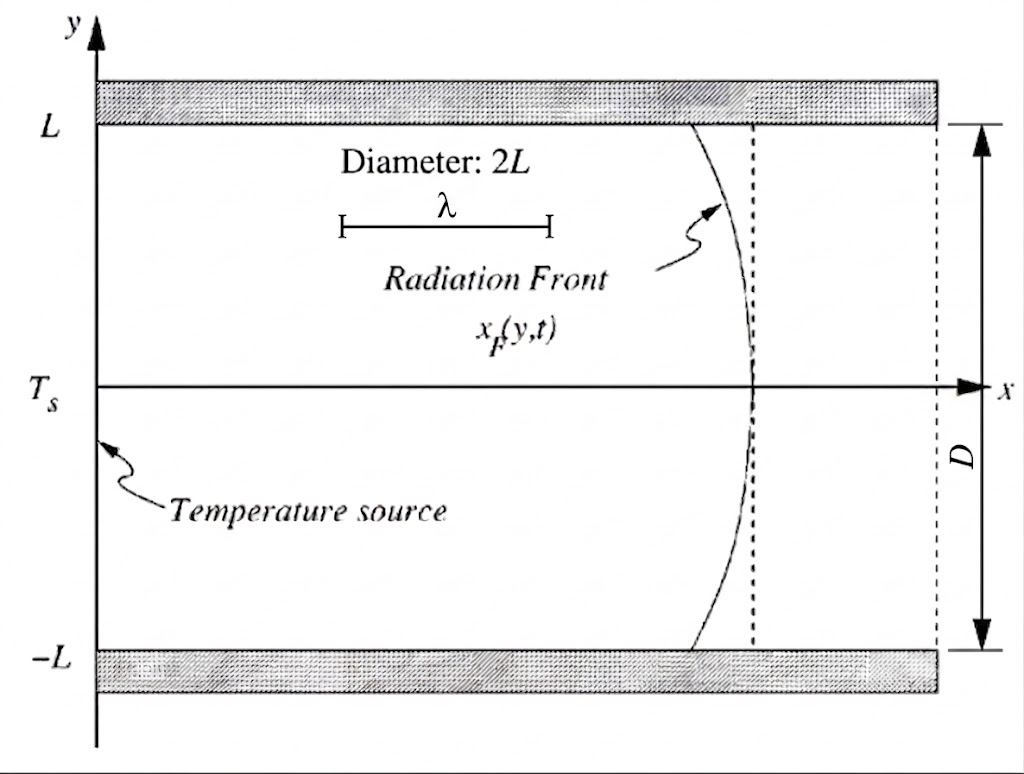
\includegraphics[width=0.95\textwidth]{figures_1.5model/lam_eff1.png}
        \end{column}
    \end{columns}
\end{frame}

\begin{frame}{Effect of the Mean Free Path Correction}
    Including the effective mean free path correction matches the model to the experimental data:
    
    \vspace{0.2cm}
    \begin{figure}
        \centering
        
\includegraphics[width=0.7\textwidth]{figures_1.5model/lam_eff.png}
    \end{figure}
\end{frame}

\begin{frame}{Comparison with Various Experiments}
    \begin{columns}
        \begin{column}{0.48\textwidth}
            \centering
                
\includegraphics[width=0.78\textwidth]{figures_1.5model/C8H7Cl.png}%
                \raisebox{2.1cm}[0pt][0pt]{\makebox[0pt][l]{\hspace{-0.7\textwidth}\fcolorbox{blue!40}{white}{\strut\scriptsize\textbf{C$_8$H$_7$Cl}}}}

            {\scriptsize \textit{Moore et al. JQSRT, (2015)}}
        \end{column}
        \begin{column}{0.48\textwidth}
            \centering
                
\includegraphics[width=0.78\textwidth]{figures_1.5model/Ta2O5.png}%
                \raisebox{1.8cm}[0pt][0pt]{\makebox[0pt][l]{\hspace{-0.69\textwidth}\fcolorbox{blue!40}{white}{\strut\scriptsize\textbf{Ta$_2$O$_5$}}}}

            {\scriptsize \textit{Back et al. POP, (2000)}}
        \end{column}
    \end{columns}
    \vspace{0.1cm}
    \begin{columns}
        \begin{column}{0.48\textwidth}
            \centering
                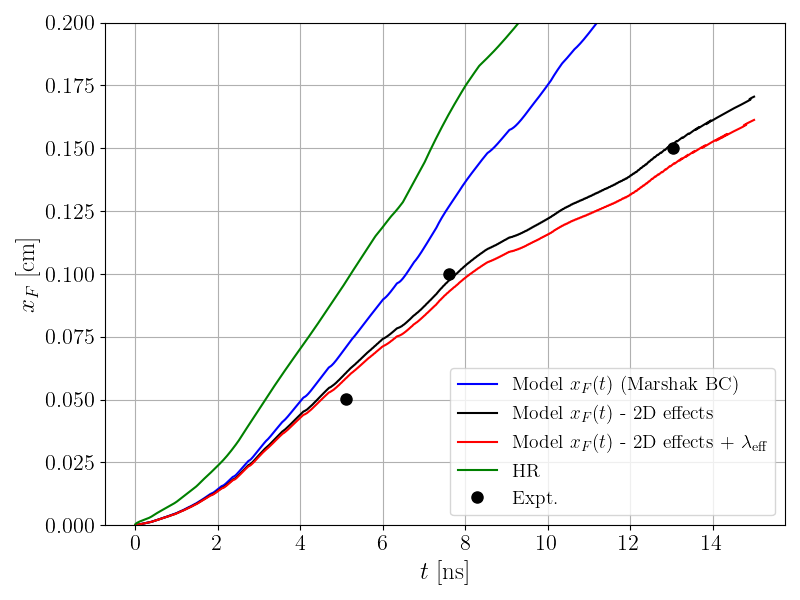
\includegraphics[width=0.78\textwidth]{figures_1.5model/SiO2_low_energy.png}%
                \raisebox{2.1cm}[0pt][0pt]{\makebox[0pt][l]{\hspace{-0.65\textwidth}\fcolorbox{blue!40}{white}{\strut\scriptsize\textbf{SiO$_2$}}}}

            {\scriptsize \textit{Back et al. PRL, (2000)}}
        \end{column}
        \begin{column}{0.48\textwidth}
            \centering
                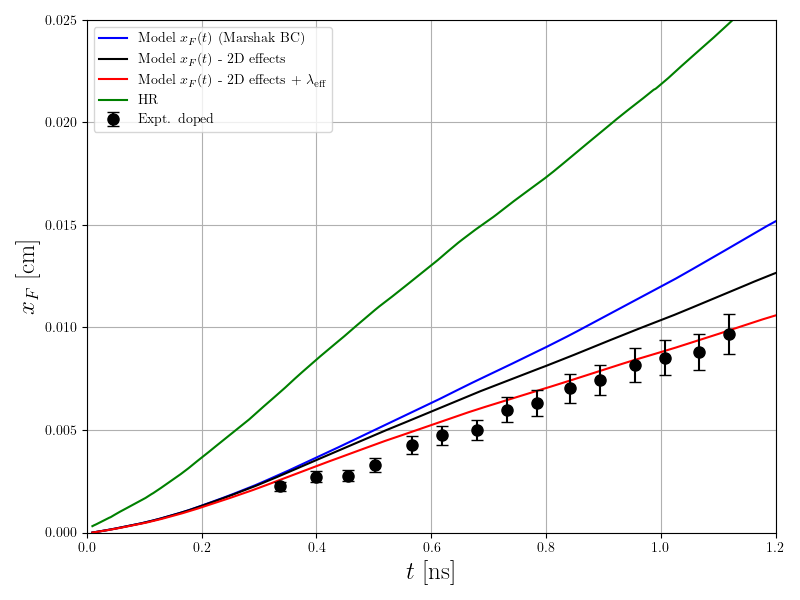
\includegraphics[width=0.78\textwidth]{figures_1.5model/Ji-Yan.png}%
                \raisebox{1.9cm}[0pt][0pt]{\makebox[0pt][l]{\hspace{-0.64\textwidth}\fcolorbox{blue!40}{white}{\strut\scriptsize\textbf{C$_8$H$_8$}}}}

            {\scriptsize \textit{Ji-Yan et al. CPB, (2010)}}
        \end{column}
    \end{columns}
\end{frame}

\begin{frame}{Flux Predicted by the Model}
    \begin{columns}
        \begin{column}{0.5\textwidth}
            Using the Henyey-like profile:
            \begin{equation*}
                T(z,t) = T_S(t) \left[ 1 - \frac{z}{z_F(t)} \right]^{\frac{1}{4+\alpha-\beta}}
            \end{equation*}
            behind the heat front ($z < z_F(t)$), and $T = 0$ ahead of it.
            
            \vspace{0.4cm}
            The radiation flux at each detector position is then computed as:
            \begin{equation*}
                \Phi(t) = \sigma_{\mathrm{SB}} T^4(z, t)
            \end{equation*}
            where the flux is computed in several different spatial locations.
        \end{column}
        \hfill
        \begin{column}{0.48\textwidth}
            \centering
            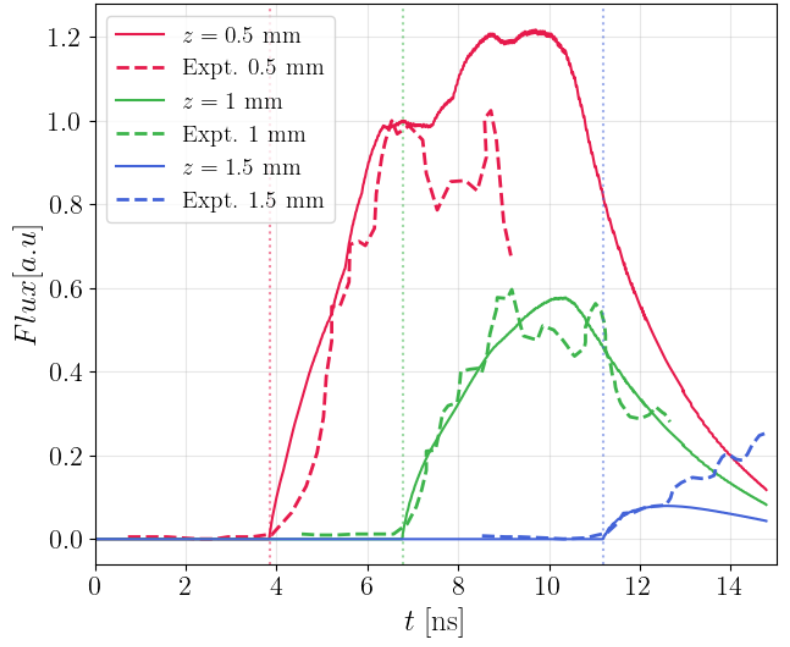
\includegraphics[width=\textwidth]{figures_1.5model/flux_back_prl.png}
        \end{column}
    \end{columns}
\end{frame}

\section{Full 2D Model}
{
\setbeamercolor{background canvas}{bg=darkblue}
\begin{frame}[plain]
    \vfill
    \begin{center}
        {\Huge\bfseries\color{white} 2D Model}
    \end{center}
    \vfill
\end{frame}
}
\subsection{Modeling the Front Curvature}
{
\setbeamercolor{background canvas}{bg=darkblue}
\begin{frame}[plain]
    \vfill
    \begin{center}
        {\color{accentblue}\LARGE Full 2D Model} \\
        \vspace{0.4cm}
        {\huge\bfseries\color{white} Modeling the Front Curvature}
    \end{center}
    \vfill
\end{frame}
}

\begin{frame}{Wall Boundary Condition}
    Non-ideal walls introduce energy loss: only a fraction $\alpha$ of incoming flux $F_{\text{in}}$ is re-emitted ($F_{\text{out}} = \alpha F_{\text{in}}$).
    \begin{columns}
        \begin{column}{0.52\textwidth}
            \begin{itemize}
                \item Net wall flux loss:
                \begin{equation*}
                    F_{\text{wall}} = (1-\alpha)F_{\text{in}} = (1-\alpha)\sigma_{\mathrm{SB}}T^4
                \end{equation*}
                \item Equating to diffusion flux (Fick's law):
                \begin{equation*}
                    F_{\text{wall}} = -\frac{4}{3}\frac{\sigma_{\mathrm{SB}}}{\rho\kappa}\frac{\partial T^4}{\partial n}
                \end{equation*}
                \item Resulting boundary condition:
                \begin{equation*}
                    \left.\frac{\partial T^4}{\partial n}\right|_{\text{wall}} = \frac{3}{4}\rho\kappa(\alpha-1)T^4\Big|_{\text{wall}}
                \end{equation*}
            \end{itemize}
        \end{column}
        \hfill
        \begin{column}{0.45\textwidth}
            \centering
            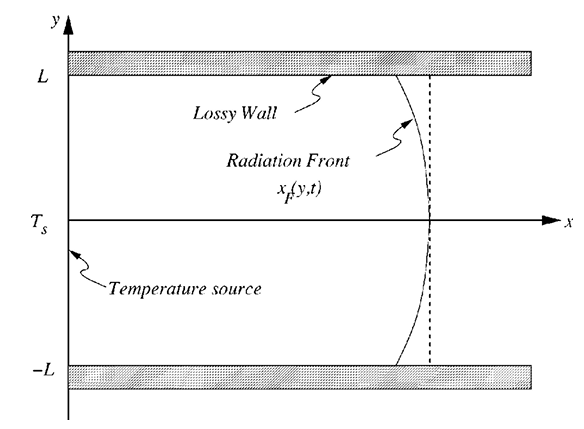
\includegraphics[height=0.5\textheight]{figures_intreduction/hurricane.png}
        \end{column}
    \end{columns}
\end{frame}

\begin{frame}{Understanding the Front Curvature}
    Hurricane \& Hammer (2006) solved the Laplace equation (assuming constant opacity and neglecting $e$):
    \begin{equation*}
        \underbrace{\frac{\partial e}{\partial t}}_{\to 0} = \frac{4}{3} \nabla \cdot \left( \frac{1}{ \rho \kappa} \nabla (T^4) \right)
    \end{equation*}
    and got the 2D front in \textcolor{blue}{\textbf{Cartesian coordinates}} (where $\varepsilon = \frac{3}{4}\rho\kappa L (1-\alpha)$):
    \begin{equation*}
        x_F(y,t) = \frac{L}{\varepsilon} \cosh^{-1}\left(1 + \frac{D\varepsilon t}{L^2}\right) \cos\left(\frac{\sqrt{\varepsilon}}{L}y\right) + \text{HOT}
    \end{equation*}
\end{frame}

\begin{frame}{Cylindrical Coordinates}
    \begin{columns}
        \begin{column}{0.65\textwidth}
            The model was re-developed in \textcolor{red}{\textbf{cylindrical coordinates}} (\textit{Courtois et al. POP, (2022)}):
            \begin{equation*}
                x_F(r,t) = \frac{1}{\kappa_0} \cosh^{-1}\left(1 + \frac{D\kappa_0^2 t}{2}\right) J_0(\kappa_0 r) + HOT
            \end{equation*}
            
            \textbf{\textcolor{blue}{Planar} $\longleftrightarrow$ \textcolor{red}{Cylindrical} Analogy}: $\cos(k y) \longleftrightarrow J_0(\kappa r)$
            \vspace{0.1cm}
            For small $\varepsilon$:
            \begin{equation*}
                \kappa_0 \approx \frac{\sqrt{2\varepsilon}}{R}, \quad \varepsilon = \frac{3}{4}\rho\kappa R (1-\alpha)
            \end{equation*}
            where $\alpha$ is the wall albedo.
        \end{column}
        \hfill
        \begin{column}{0.35\textwidth}
            \centering
            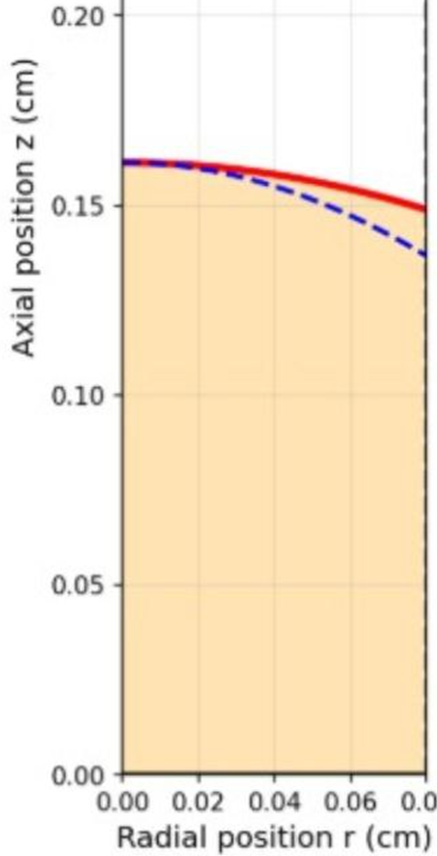
\includegraphics[width=0.7\textwidth]{2D_model/cylinder_vs_cartezian.png}
        \end{column}
    \end{columns}
\end{frame}

\begin{frame}{Applying to Our Model: Dynamic Albedo}
    In previous works, the wall albedo was treated as a constant fitting parameter. We update it dynamically over time:
    \begin{equation*}
        \alpha(t) = \frac{F_{\text{out, wall}}}{F_{\text{in,wall}}} = \frac{\sigma_{\mathrm{SB}}T_{s,\mathrm{interface}}^4 - \frac{dE_{\text{wall}}}{dt}/2}{\sigma_{\mathrm{SB}}T_{s,\mathrm{interface}}^4+\frac{dE_{\text{wall}}}{dt}/2}
    \end{equation*}
    
    \vspace{0.4cm}
    \begin{columns}
        \begin{column}{0.55\textwidth}
            where the front curvature depends on the radial eigenvalue $\kappa_0$:
            \begin{equation*}
                \kappa_0(t) \approx \frac{\sqrt{2\varepsilon(t)}}{R}, \quad \varepsilon(t) = \frac{3}{4}\rho\kappa R (1-\alpha(t))
            \end{equation*}
            which dynamically scales with the time-dependent wall loss $(1 - \alpha(t))$.
        \end{column}
        \hfill
        \begin{column}{0.42\textwidth}
            \centering
            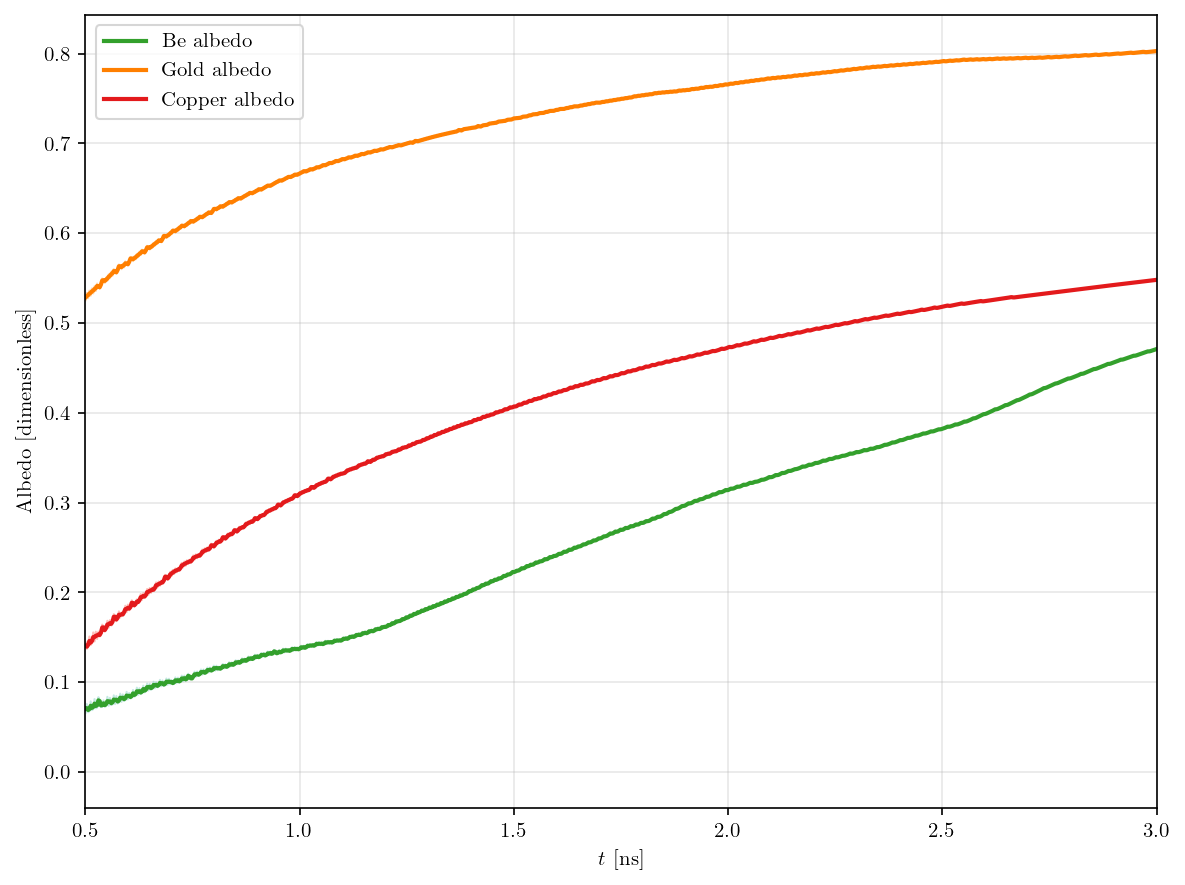
\includegraphics[width=\textwidth]{2D_model/albedo.png}
        \end{column}
    \end{columns}
\end{frame}

\begin{frame}{The 2D Wave Front}
    {\LARGE
    \begin{equation*}
        \boldsymbol{x_F(r,t) = x_{\text{1.5D}}(t) \cdot J_0\left(\kappa_0 (t) r\right)}
    \end{equation*}
    }

\end{frame}



\subsection{Comparing to 2D Supersonic Diffusion Simulation}
{
\setbeamercolor{background canvas}{bg=darkblue}
\begin{frame}[plain]
    \vfill
    \begin{center}
        {\color{accentblue}\LARGE Full 2D Model} \\
        \vspace{0.4cm}
        {\huge\bfseries\color{white} Comparing to 2D Diffusion Simulation Without Hydrodynamics}
    \end{center}
    \vfill
\end{frame}
}


\begin{frame}{Gold Coating — \(\mathrm{SiO}_2\)}
    \begin{figure}
        \centering
            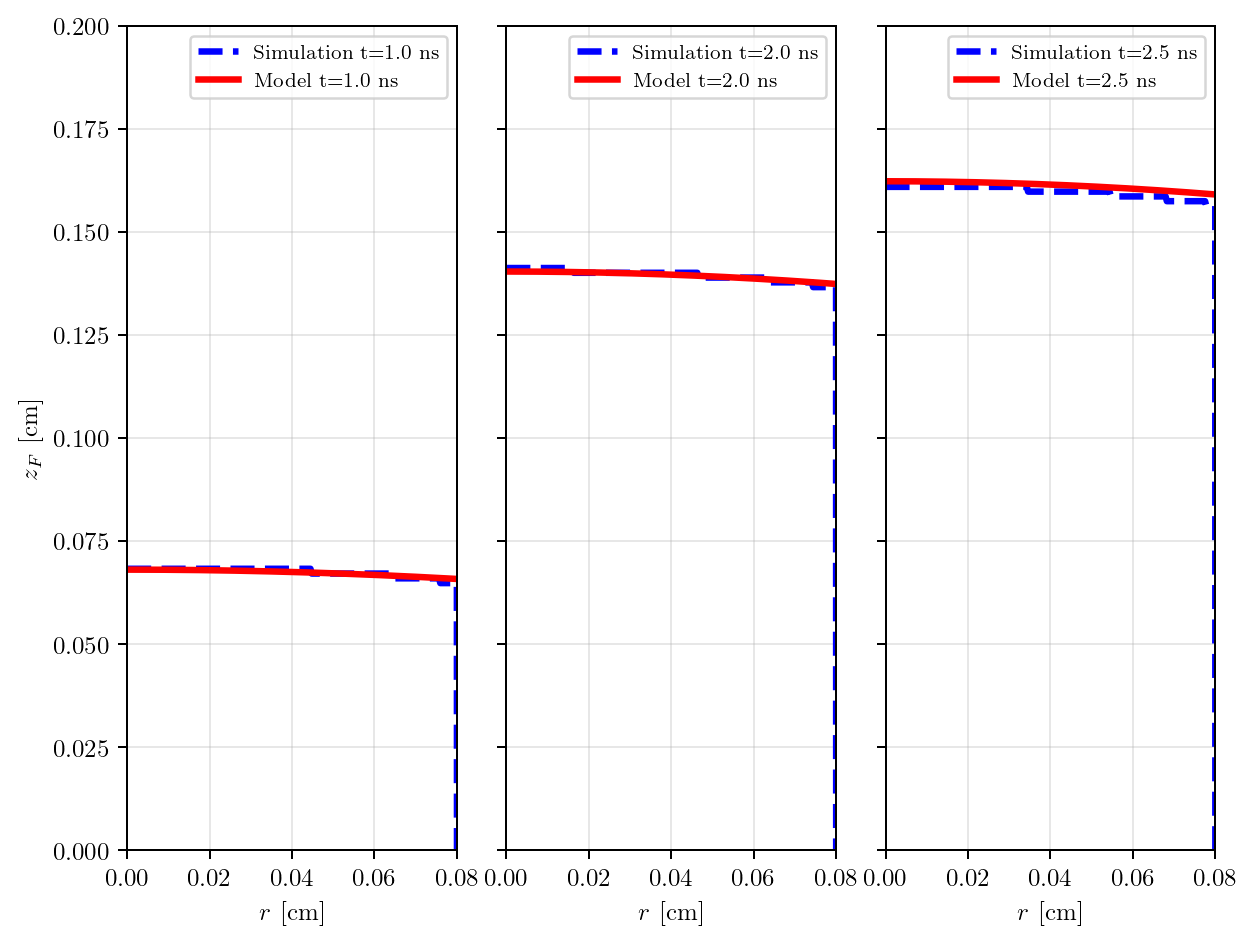
\includegraphics[width=0.8\textwidth]{2D_model/front_surface_gold.png}
    \end{figure}
\end{frame}

\begin{frame}{100$\times$ Optically Thinner Gold Coating — \(\mathrm{SiO}_2\)}
    \begin{figure}
        \centering
        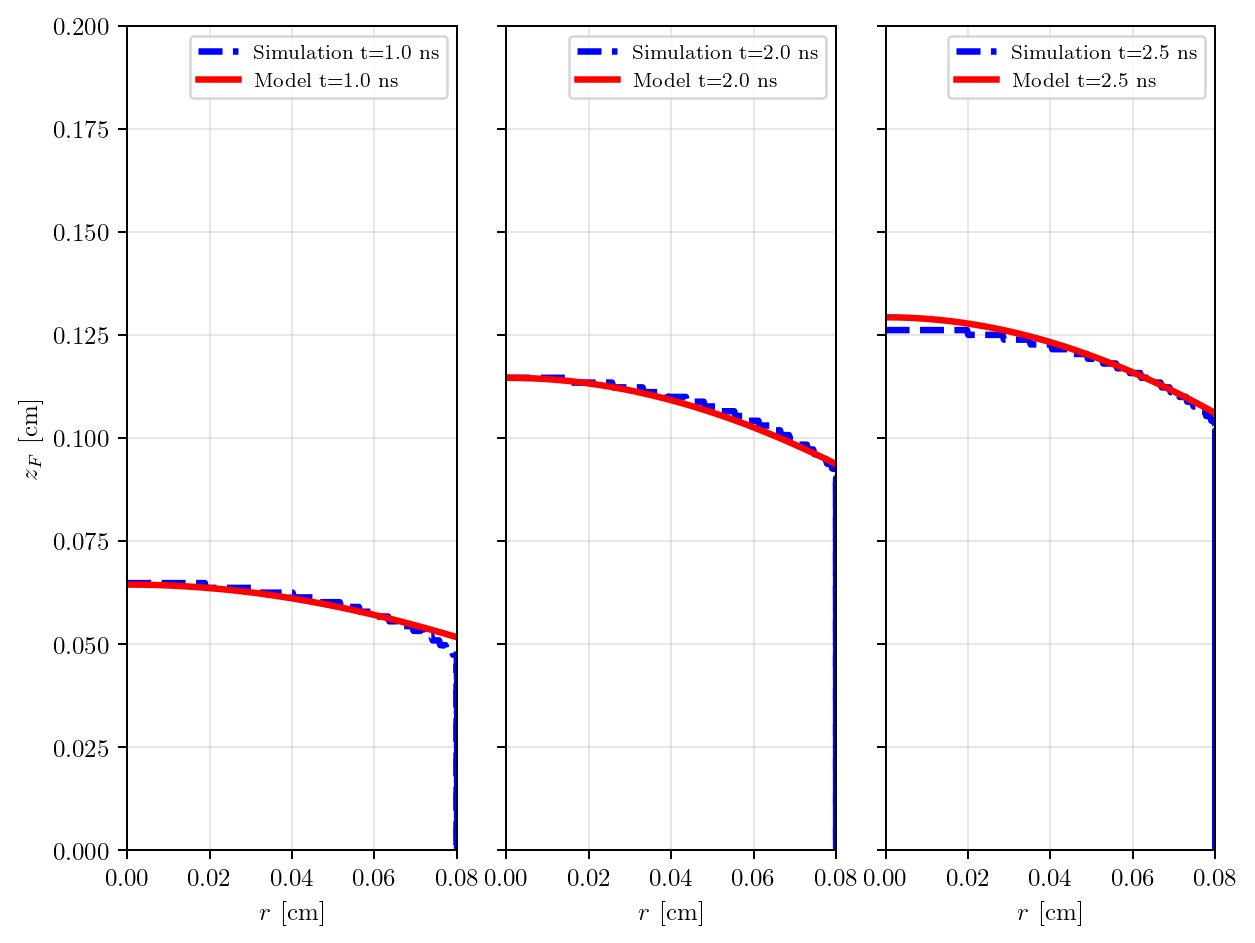
\includegraphics[width=0.8\textwidth]{2D_model/front_surface_gold100.png}
    \end{figure}
\end{frame}

\begin{frame}{Copper Coating — \(\mathrm{SiO}_2\)}
    \begin{figure}
        \centering
        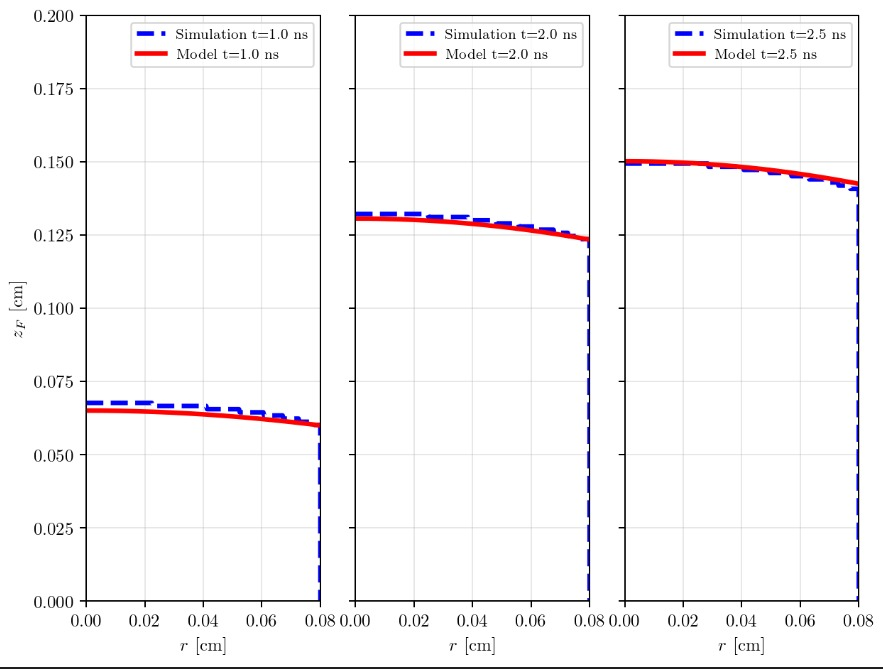
\includegraphics[width=0.8\textwidth]{2D_model/front_surface_copper.png}
    \end{figure}
\end{frame}

\begin{frame}{Beryllium (Be) Coating — \(\mathrm{SiO}_2\)}
    \begin{figure}
        \centering
        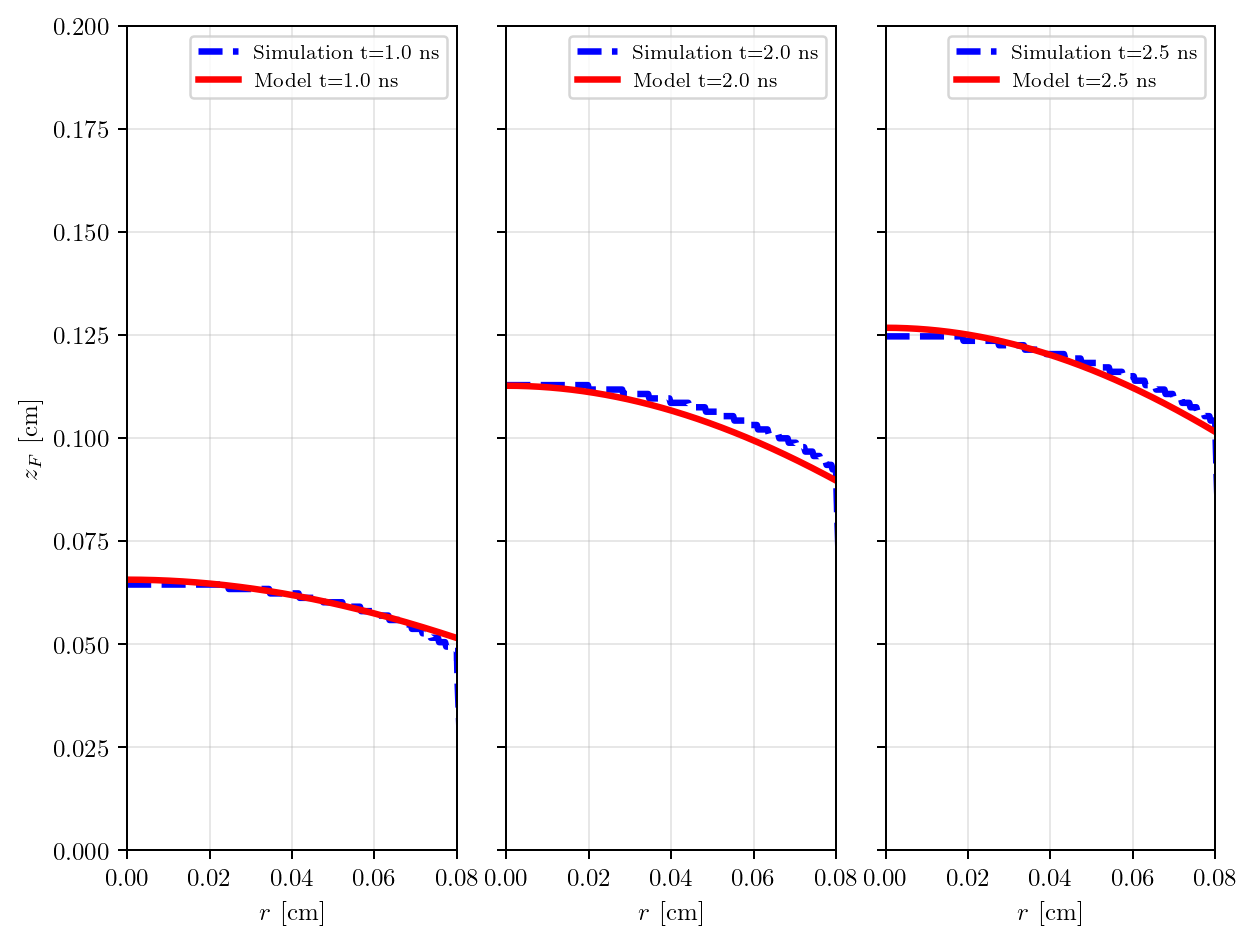
\includegraphics[width=0.8\textwidth]{2D_model/front_surface_be.png}
    \end{figure}
\end{frame}

\begin{frame}{Vacuum Boundary — \(\mathrm{SiO}_2\)}
    \begin{figure}
        \centering
        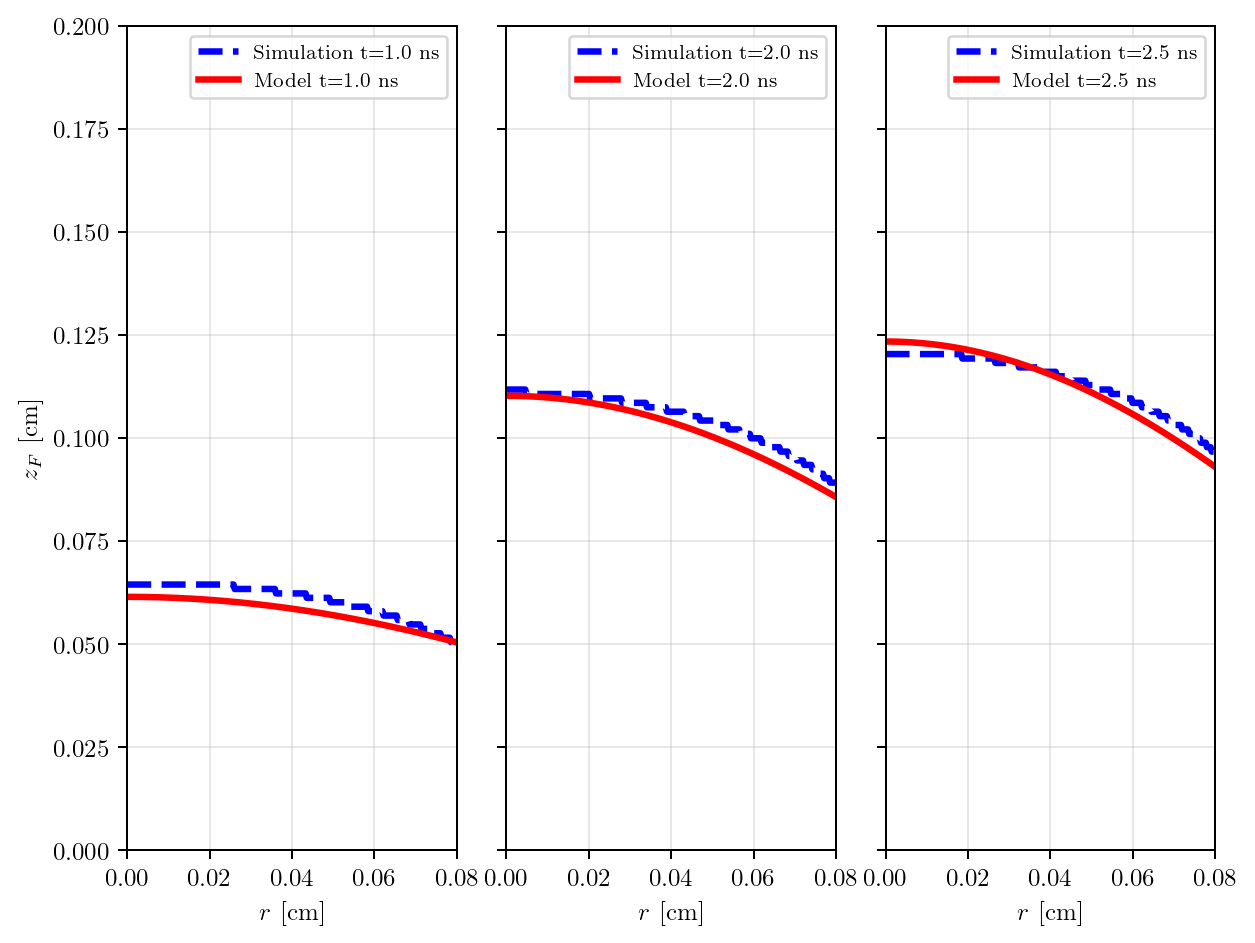
\includegraphics[width=0.8\textwidth]{2D_model/front_surface_vacuum.png}
    \end{figure}
\end{frame}

\subsection{Full 2D Temperature Distribution}
{
\setbeamercolor{background canvas}{bg=darkblue}
\begin{frame}[plain]
    \vfill
    \begin{center}
        {\color{accentblue}\LARGE Full 2D Model} \\
        \vspace{0.4cm}
        {\huge\bfseries\color{white} A Full 2D Temperature Distribution}
    \end{center}
    \vfill
\end{frame}
}

\begin{frame}{Full 2D Temperature Distribution}
    The 2D Henyey-like temperature profile is given by:
    \begin{equation*}
        T(z,r,t) \approx T_S(t) \left[ 1 - \frac{z}{z_F(r,t)} \right]^{\frac{1}{4+\alpha-\beta}}
    \end{equation*}

    \vspace{0.3cm}
    \begin{columns}
        \begin{column}{0.3\textwidth}
            \centering
            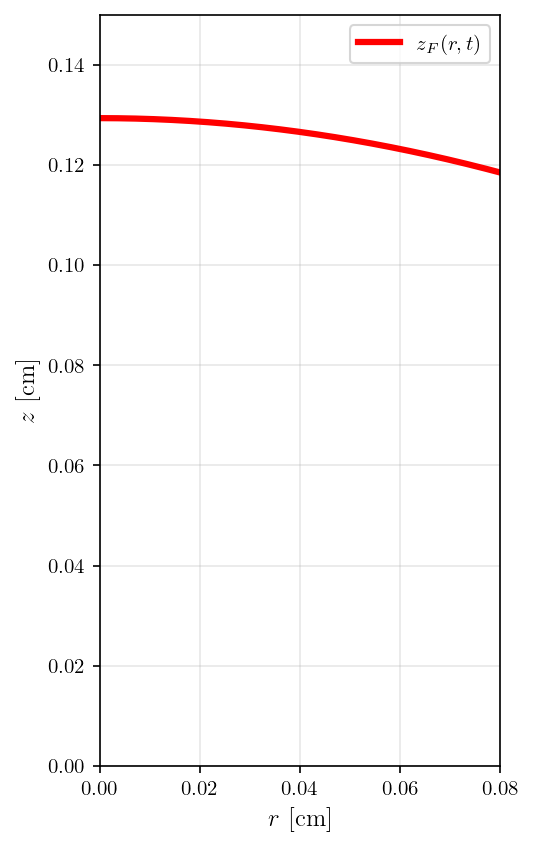
\includegraphics[width=\textwidth]{2D_model/2D_front_spatial.png} \\
            \vspace{0.1cm}
        \end{column}
        \begin{column}{0.12\textwidth}
            \centering
            \Huge $\Rightarrow$
        \end{column}
        \begin{column}{0.35\textwidth}
            \centering
            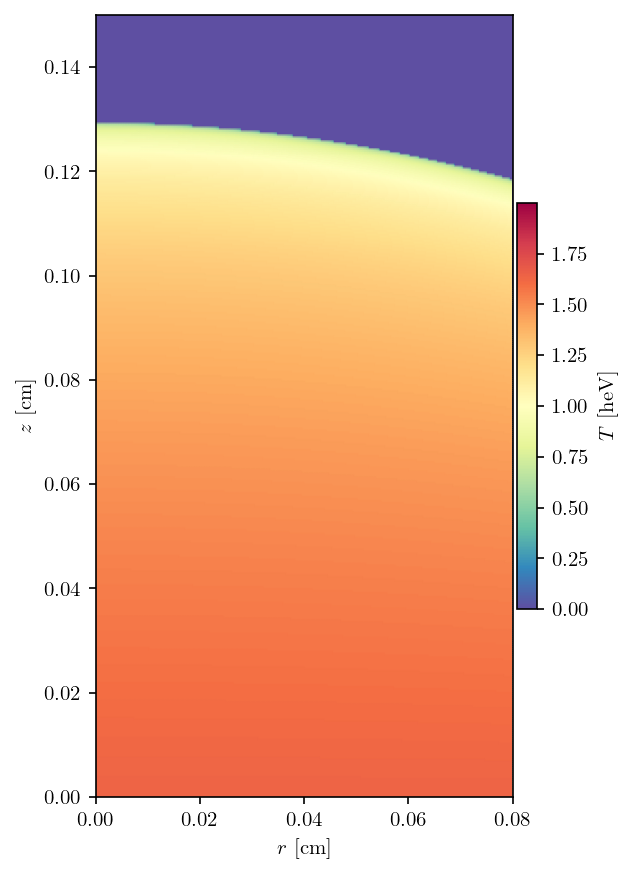
\includegraphics[width=\textwidth]{2D_model/temperature_heatmap_2D(gold wall loss).png} \\
            \vspace{0.1cm}
        \end{column}
    \end{columns}
\end{frame}

\begin{frame}{2D Temperature Distribution — Moore ($\mathrm{C}_8\mathrm{H}_7\mathrm{Cl}$)}
    \begin{columns}
        \begin{column}{0.4\textwidth}
                Side-by-side comparison of the 2D temperature distribution at $t = 3.72$ ns:
                \begin{itemize}
                    \item \textbf{Left}: Diffusion simulation with hydrodynamics taken from \textit{Moore et al. JQSRT, (2015)}.
                    \item \textbf{Right}: Our full 2D model.
                \end{itemize}
                \begin{figure}
                    \centering
                    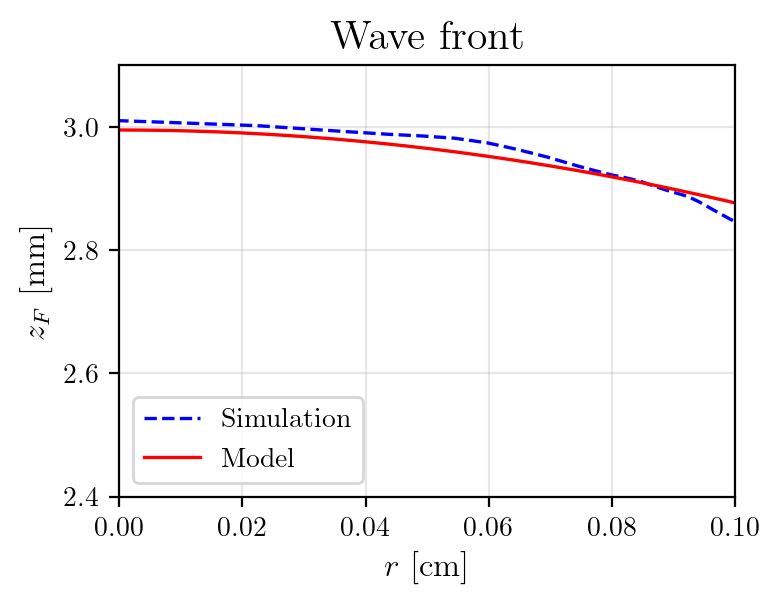
\includegraphics[width=0.8\textwidth]{2D_model/front_comparison_3.72ns.png}
                \end{figure}
        \end{column}
        \begin{column}{0.6\textwidth}
            \centering
            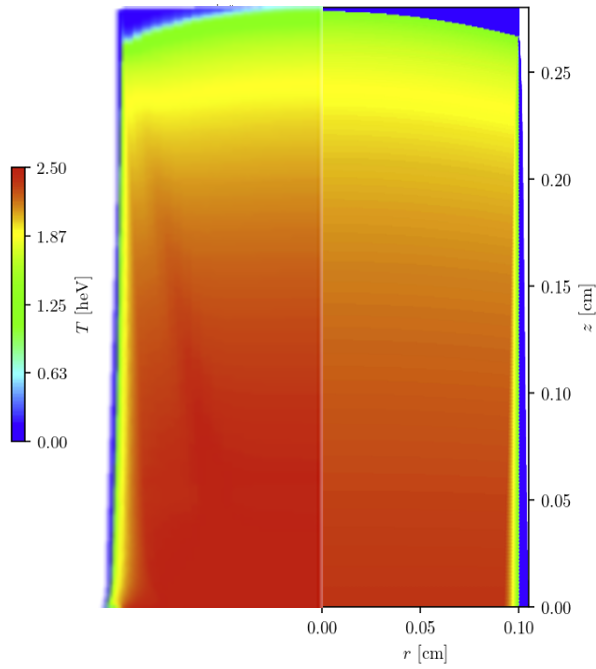
\includegraphics[height=0.9\textheight]{2D_model/moore_simulation.png}
        \end{column}
    \end{columns}
\end{frame}

\begin{frame}{2D Temperature Distribution — Back \textit{et al.} \(\mathrm{SiO}_2\) ($1.0$ ns)}
    \begin{columns}
        \begin{column}{0.4\textwidth}
                Side-by-side comparison of the 2D temperature distribution at $t = 1.0$ ns:
                \begin{itemize}
                    \item \textbf{Left}: Implicit Monte Carlo (IMC) simulation from \textit{Cohen et al. PRR, (2020)}.
                    \item \textbf{Right}: Our full 2D model with $\lambda_{\text{eff}} = 1.5$ correction.
                \end{itemize}
        \end{column}
        \begin{column}{0.6\textwidth}
            \centering
            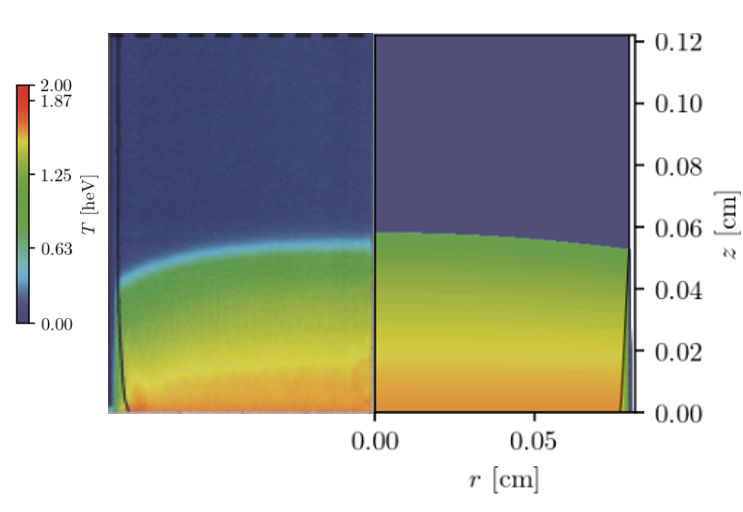
\includegraphics[height=0.55\textheight]{2D_model/back_1ns.png}
        \end{column}
    \end{columns}
\end{frame}

\begin{frame}{2D Temperature Distribution — Back \textit{et al.} \(\mathrm{SiO}_2\) ($2.0$ ns)}
    \begin{columns}
        \begin{column}{0.4\textwidth}
                Side-by-side comparison of the 2D temperature distribution at $t = 2.0$ ns:
                \begin{itemize}
                    \item \textbf{Left}: Implicit Monte Carlo (IMC) simulation from \textit{Cohen et al. PRR, (2020)}.
                    \item \textbf{Right}: Our full 2D model with $\lambda_{\text{eff}} = 1.5$ correction.
                \end{itemize}
        \end{column}
        \begin{column}{0.6\textwidth}
            \centering
            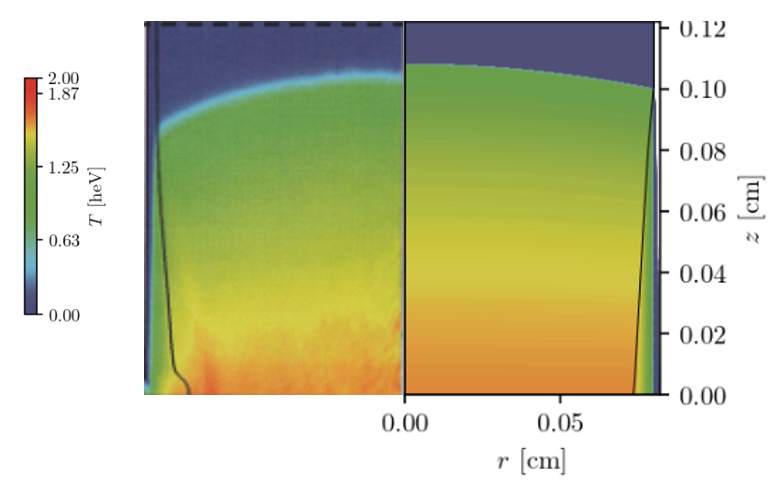
\includegraphics[height=0.5\textheight]{2D_model/back_2ns.png}
        \end{column}
    \end{columns}
\end{frame}

\begin{frame}{2D Temperature Distribution — Back \textit{et al.} \(\mathrm{SiO}_2\) ($2.5$ ns)}
    \begin{columns}
        \begin{column}{0.4\textwidth}
                Side-by-side comparison of the 2D temperature distribution at $t = 2.5$ ns:
                \begin{itemize}
                    \item \textbf{Left}: Implicit Monte Carlo (IMC) simulation from \textit{Cohen et al. PRR, (2020)}.
                    \item \textbf{Right}: Our full 2D model with $\lambda_{\text{eff}} = 1.5$ correction.
                \end{itemize}
        \end{column}
        \begin{column}{0.6\textwidth}
            \centering
            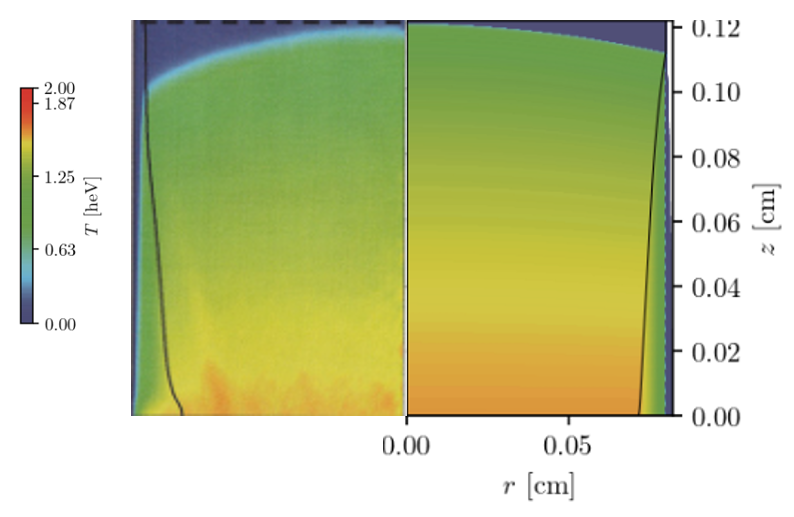
\includegraphics[height=0.53\textheight]{2D_model/back_2.5ns.png}
        \end{column}
    \end{columns}
\end{frame}

\begin{frame}{2D Temperature Distribution — Ji-Yan ($0.5$ ns)}
    \begin{columns}
        \begin{column}{0.4\textwidth}
                Side-by-side comparison of the 2D temperature distribution at $t = 0.5$ ns:
                \begin{itemize}
                    \item \textbf{Left}: 2D supersonic diffusion simulation of \textit{Ji-Yan et al. CPB, (2010)} experiment.
                    \item \textbf{Right}: Our full 2D model.
                \end{itemize}
                \begin{figure}
                    \centering
                    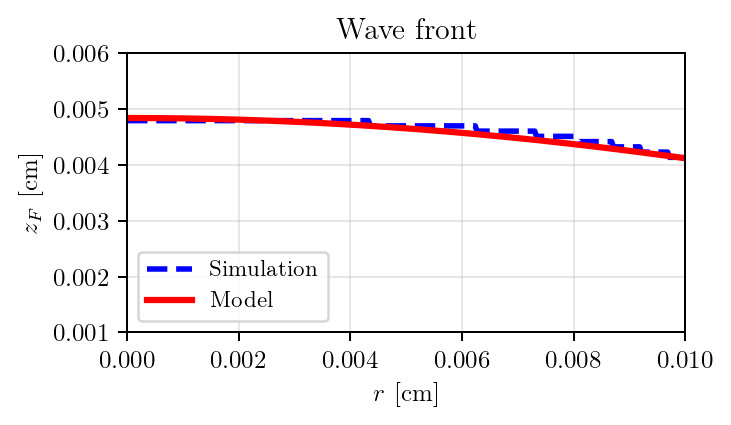
\includegraphics[width=1.05\textwidth]{2D_model/Ji-Yan_0.5ns_front.png}
                \end{figure}
        \end{column}
        \begin{column}{0.6\textwidth}
            \centering
            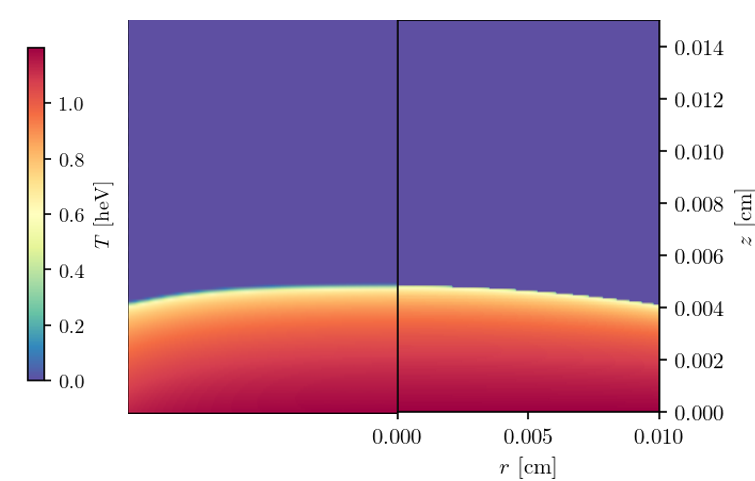
\includegraphics[height=0.49\textheight]{2D_model/Ji-Yan_0.5ns.png}
        \end{column}
    \end{columns}
\end{frame}

\begin{frame}{2D Temperature Distribution — Ji-Yan ($1.0$ ns)}
    \begin{columns}
        \begin{column}{0.4\textwidth}
                Side-by-side comparison of the 2D temperature distribution at $t = 1.0$ ns:
                \begin{itemize}
                    \item \textbf{Left}: 2D supersonic diffusion simulation of \textit{Ji-Yan et al. CPB, (2010)} experiment.
                    \item \textbf{Right}: Our full 2D model.
                \end{itemize}
                \begin{figure}
                    \centering
                    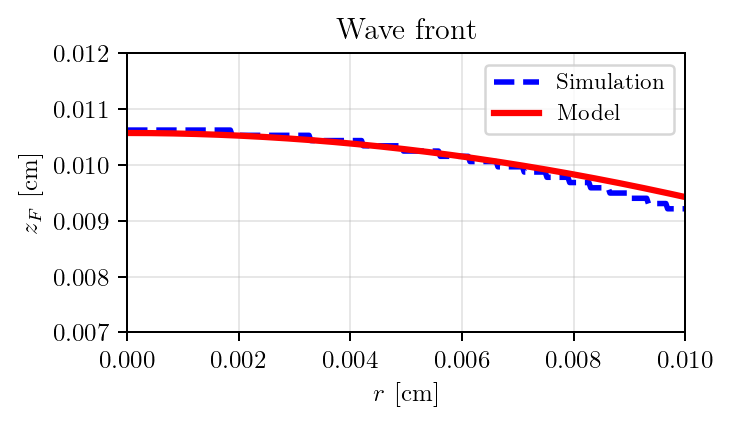
\includegraphics[width=1.05\textwidth]{2D_model/Ji-Yan_1ns_front.png}
                \end{figure}
        \end{column}
        \begin{column}{0.6\textwidth}
            \centering
            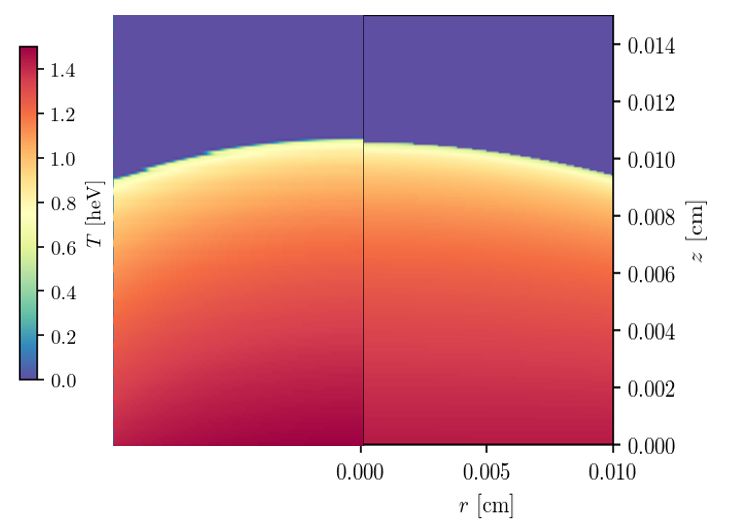
\includegraphics[height=0.55\textheight]{2D_model/Ji-Yan_1ns.png}
        \end{column}
    \end{columns}
\end{frame}

\begin{frame}{2D Temperature Distribution — Ji-Yan ($1.3$ ns)}
    \begin{columns}
        \begin{column}{0.4\textwidth}
                Side-by-side comparison of the 2D temperature distribution at $t = 1.3$ ns:
                \begin{itemize}
                    \item \textbf{Left}: 2D supersonic diffusion simulation of \textit{Ji-Yan et al. CPB, (2010)} experiment.
                    \item \textbf{Right}: Our full 2D model.
                \end{itemize}
                \begin{figure}
                    \centering
                    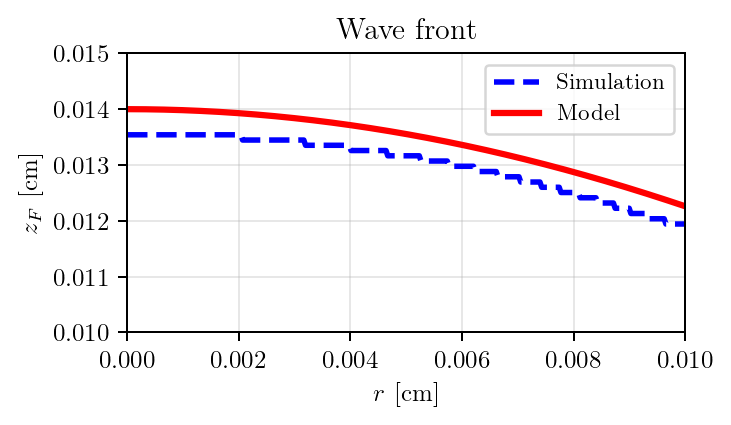
\includegraphics[width=1.05\textwidth]{2D_model/Ji-Yan_1.3ns_front.png}
                \end{figure}
        \end{column}
        \begin{column}{0.6\textwidth}
            \centering
            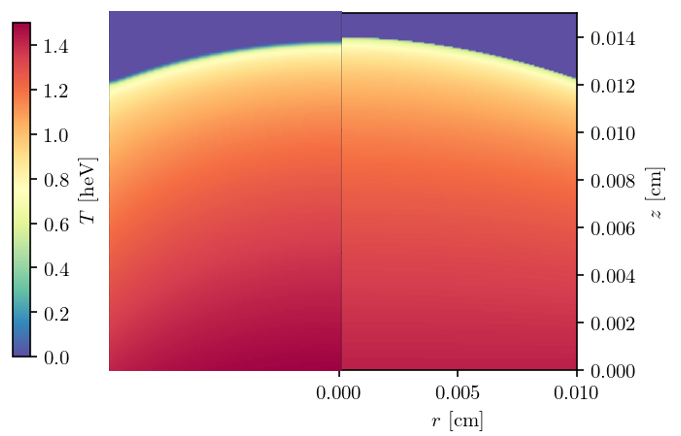
\includegraphics[height=0.55\textheight]{2D_model/Ji-Yan_1.3ns.png}
        \end{column}
    \end{columns}
\end{frame}

\subsection{Comparison with Experimental Data}

{
\setbeamercolor{background canvas}{bg=darkblue}
\begin{frame}[plain]
    \vfill
    \begin{center}
        {\color{accentblue}\LARGE Full 2D Model} \\
        \vspace{0.4cm}
        {\huge\bfseries\color{white} Comparison with Experimental Data}
    \end{center}
    \vfill
\end{frame}
}

\begin{frame}{Flux Curvature Comparison — Back \textit{et al.} \(\mathrm{SiO}_2\) (PRL)}
    \begin{columns}
        \begin{column}{0.37\textwidth}
            \centering
            
\includegraphics[width=\textwidth]{2D_model/prl_T4.png} \\
            \vspace{0.2cm}
            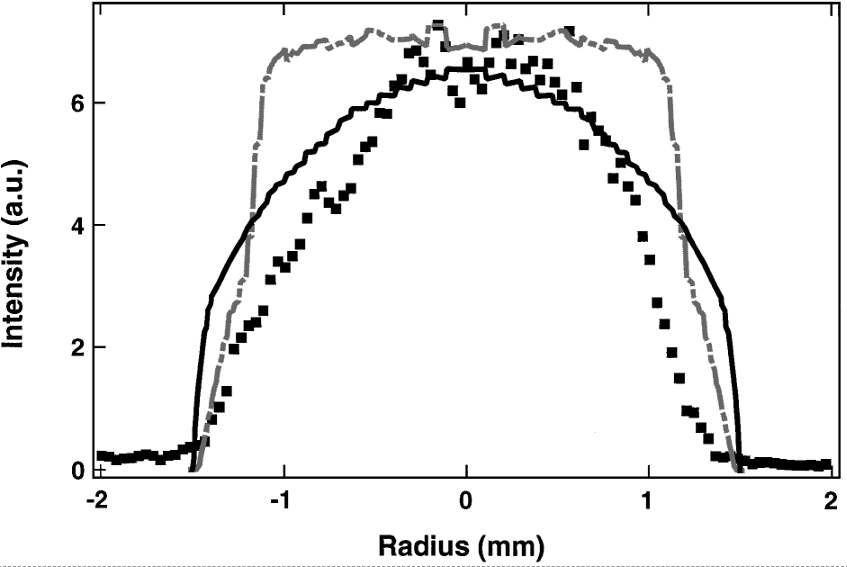
\includegraphics[width=0.9\textwidth]{2D_model/prl.png}
            {\scriptsize \textit{Back et al. PRL, (2000)}}
        \end{column}
        \begin{column}{0.1\textwidth}
            \centering
            \Huge $\Rightarrow$
        \end{column}
        \begin{column}{0.6\textwidth}
            \centering
            
\includegraphics[width=\textwidth]{2D_model/back_prl_curve.png}
        \end{column}
    \end{columns}
\end{frame}

\begin{frame}{Flux Curvature Comparison — Back \textit{et al.} \(\mathrm{Ta}_2\mathrm{O}_5\) (POP)}
    \begin{columns}
        \begin{column}{0.37\textwidth}
            \centering
            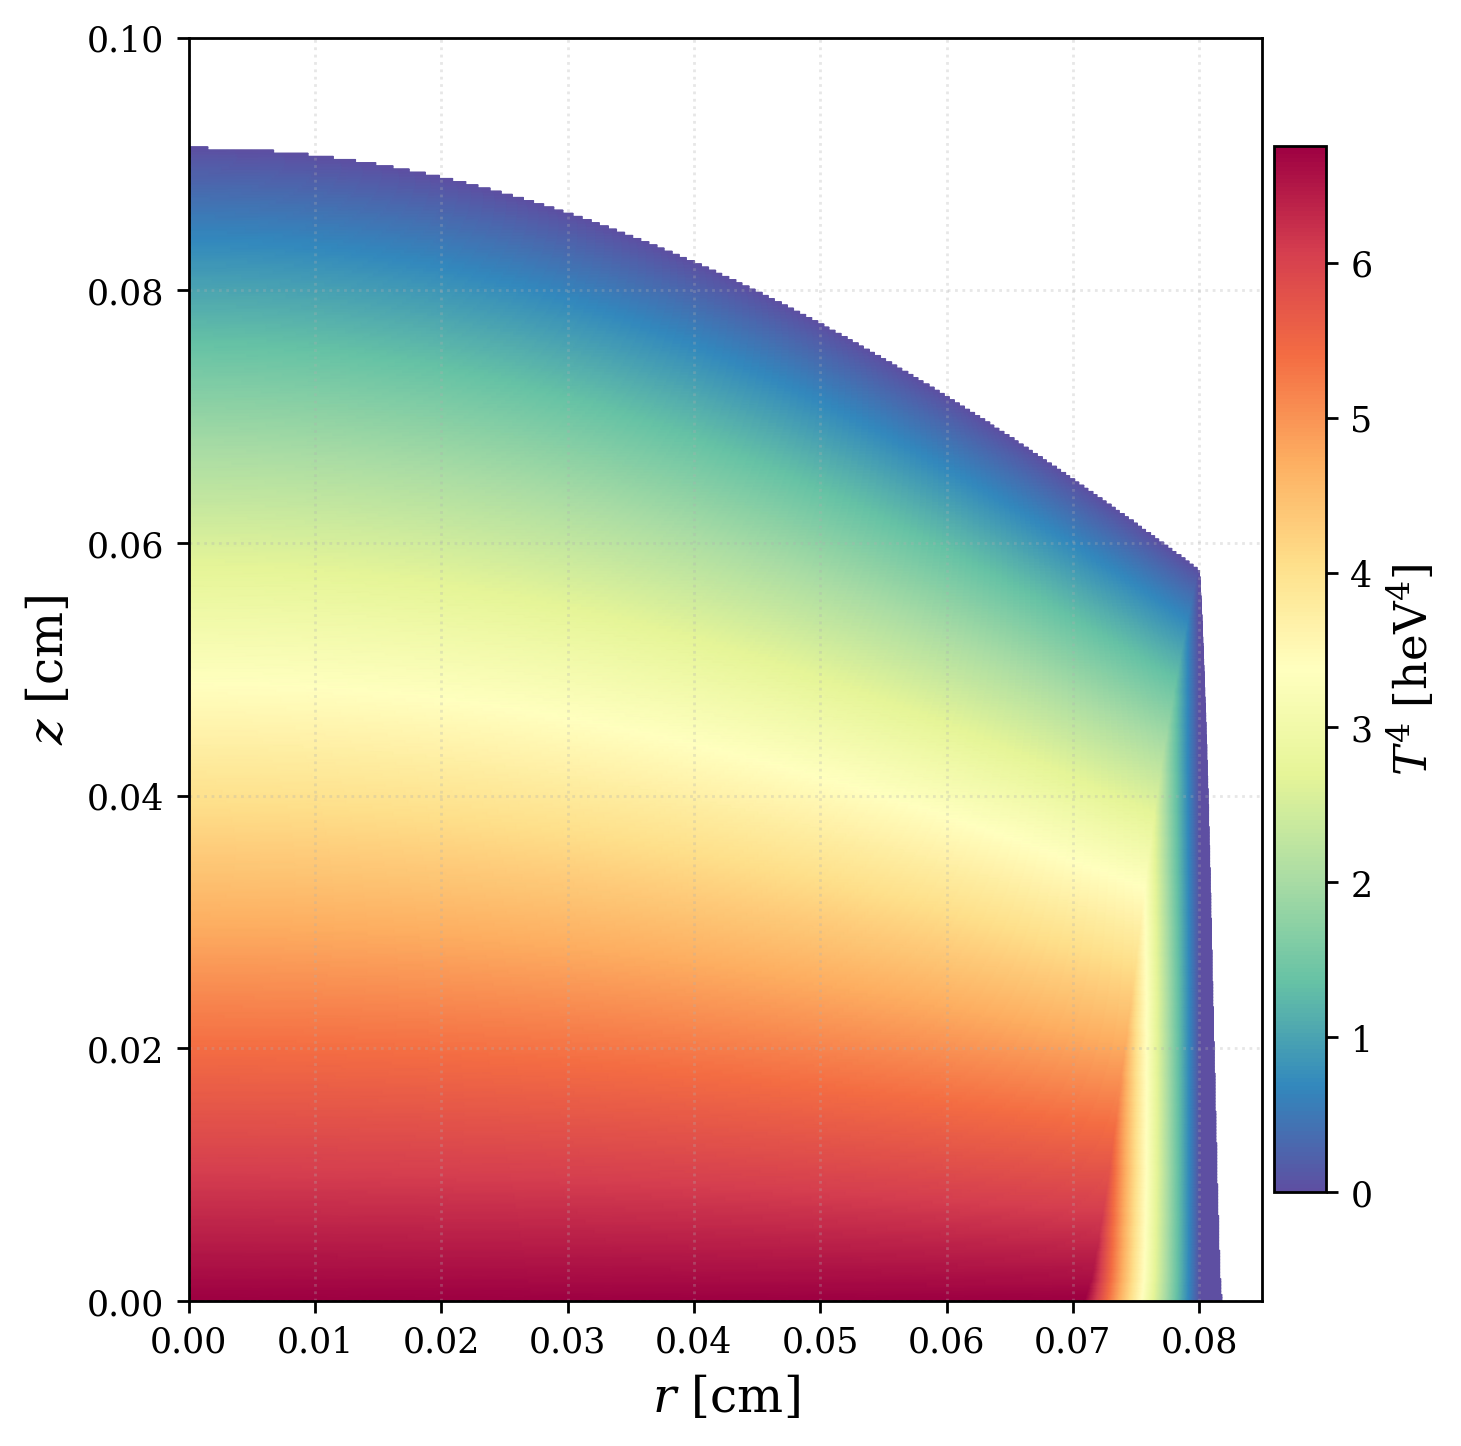
\includegraphics[width=\textwidth]{2D_model/T4_spatial_heatmap_2.0ns.png} \\
            \vspace{0.2cm}
            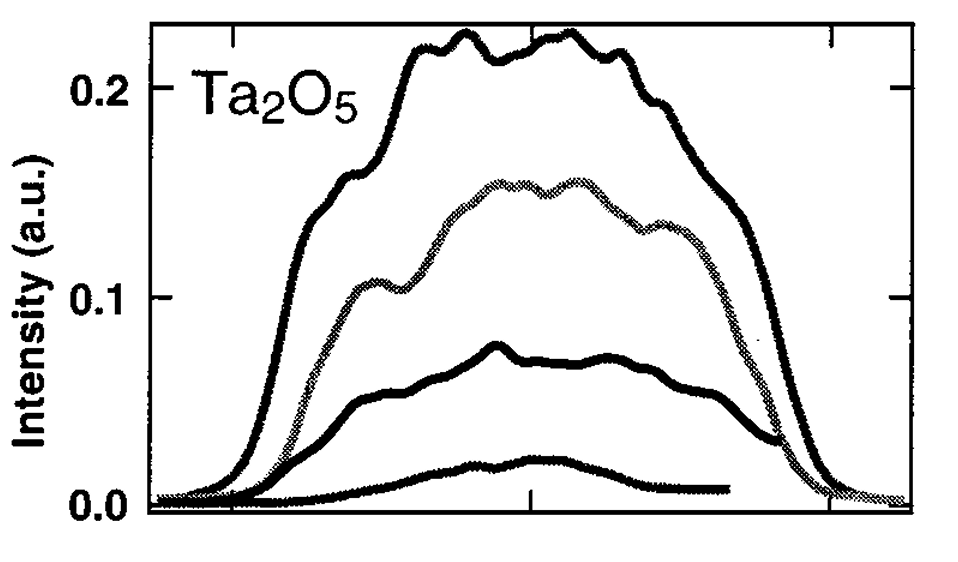
\includegraphics[width=0.9\textwidth]{2D_model/Ta2O5_intensity.png}
            {\scriptsize \textit{Back et al. POP, (2000)}}
        \end{column}
        \begin{column}{0.1\textwidth}
            \centering
            \Huge $\Rightarrow$
        \end{column}
        \begin{column}{0.6\textwidth}
            \centering
            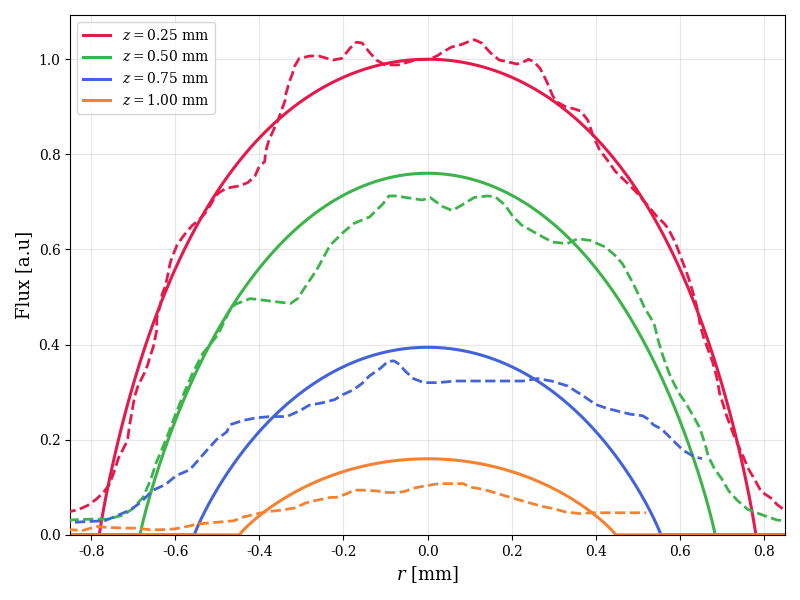
\includegraphics[width=\textwidth]{2D_model/flux_curvature_post_breakout_0.5ns.png}
        \end{column}
    \end{columns}
\end{frame}

\begin{frame}{Gold vs. Copper Coating Comparison}
    Comparison with the French experiment by \textit{Courtois et al. POP, (2024)}, measuring the front arrival time as a function of $r$ for both gold and copper coatings:
    \vfill
    \begin{figure}
        \centering
        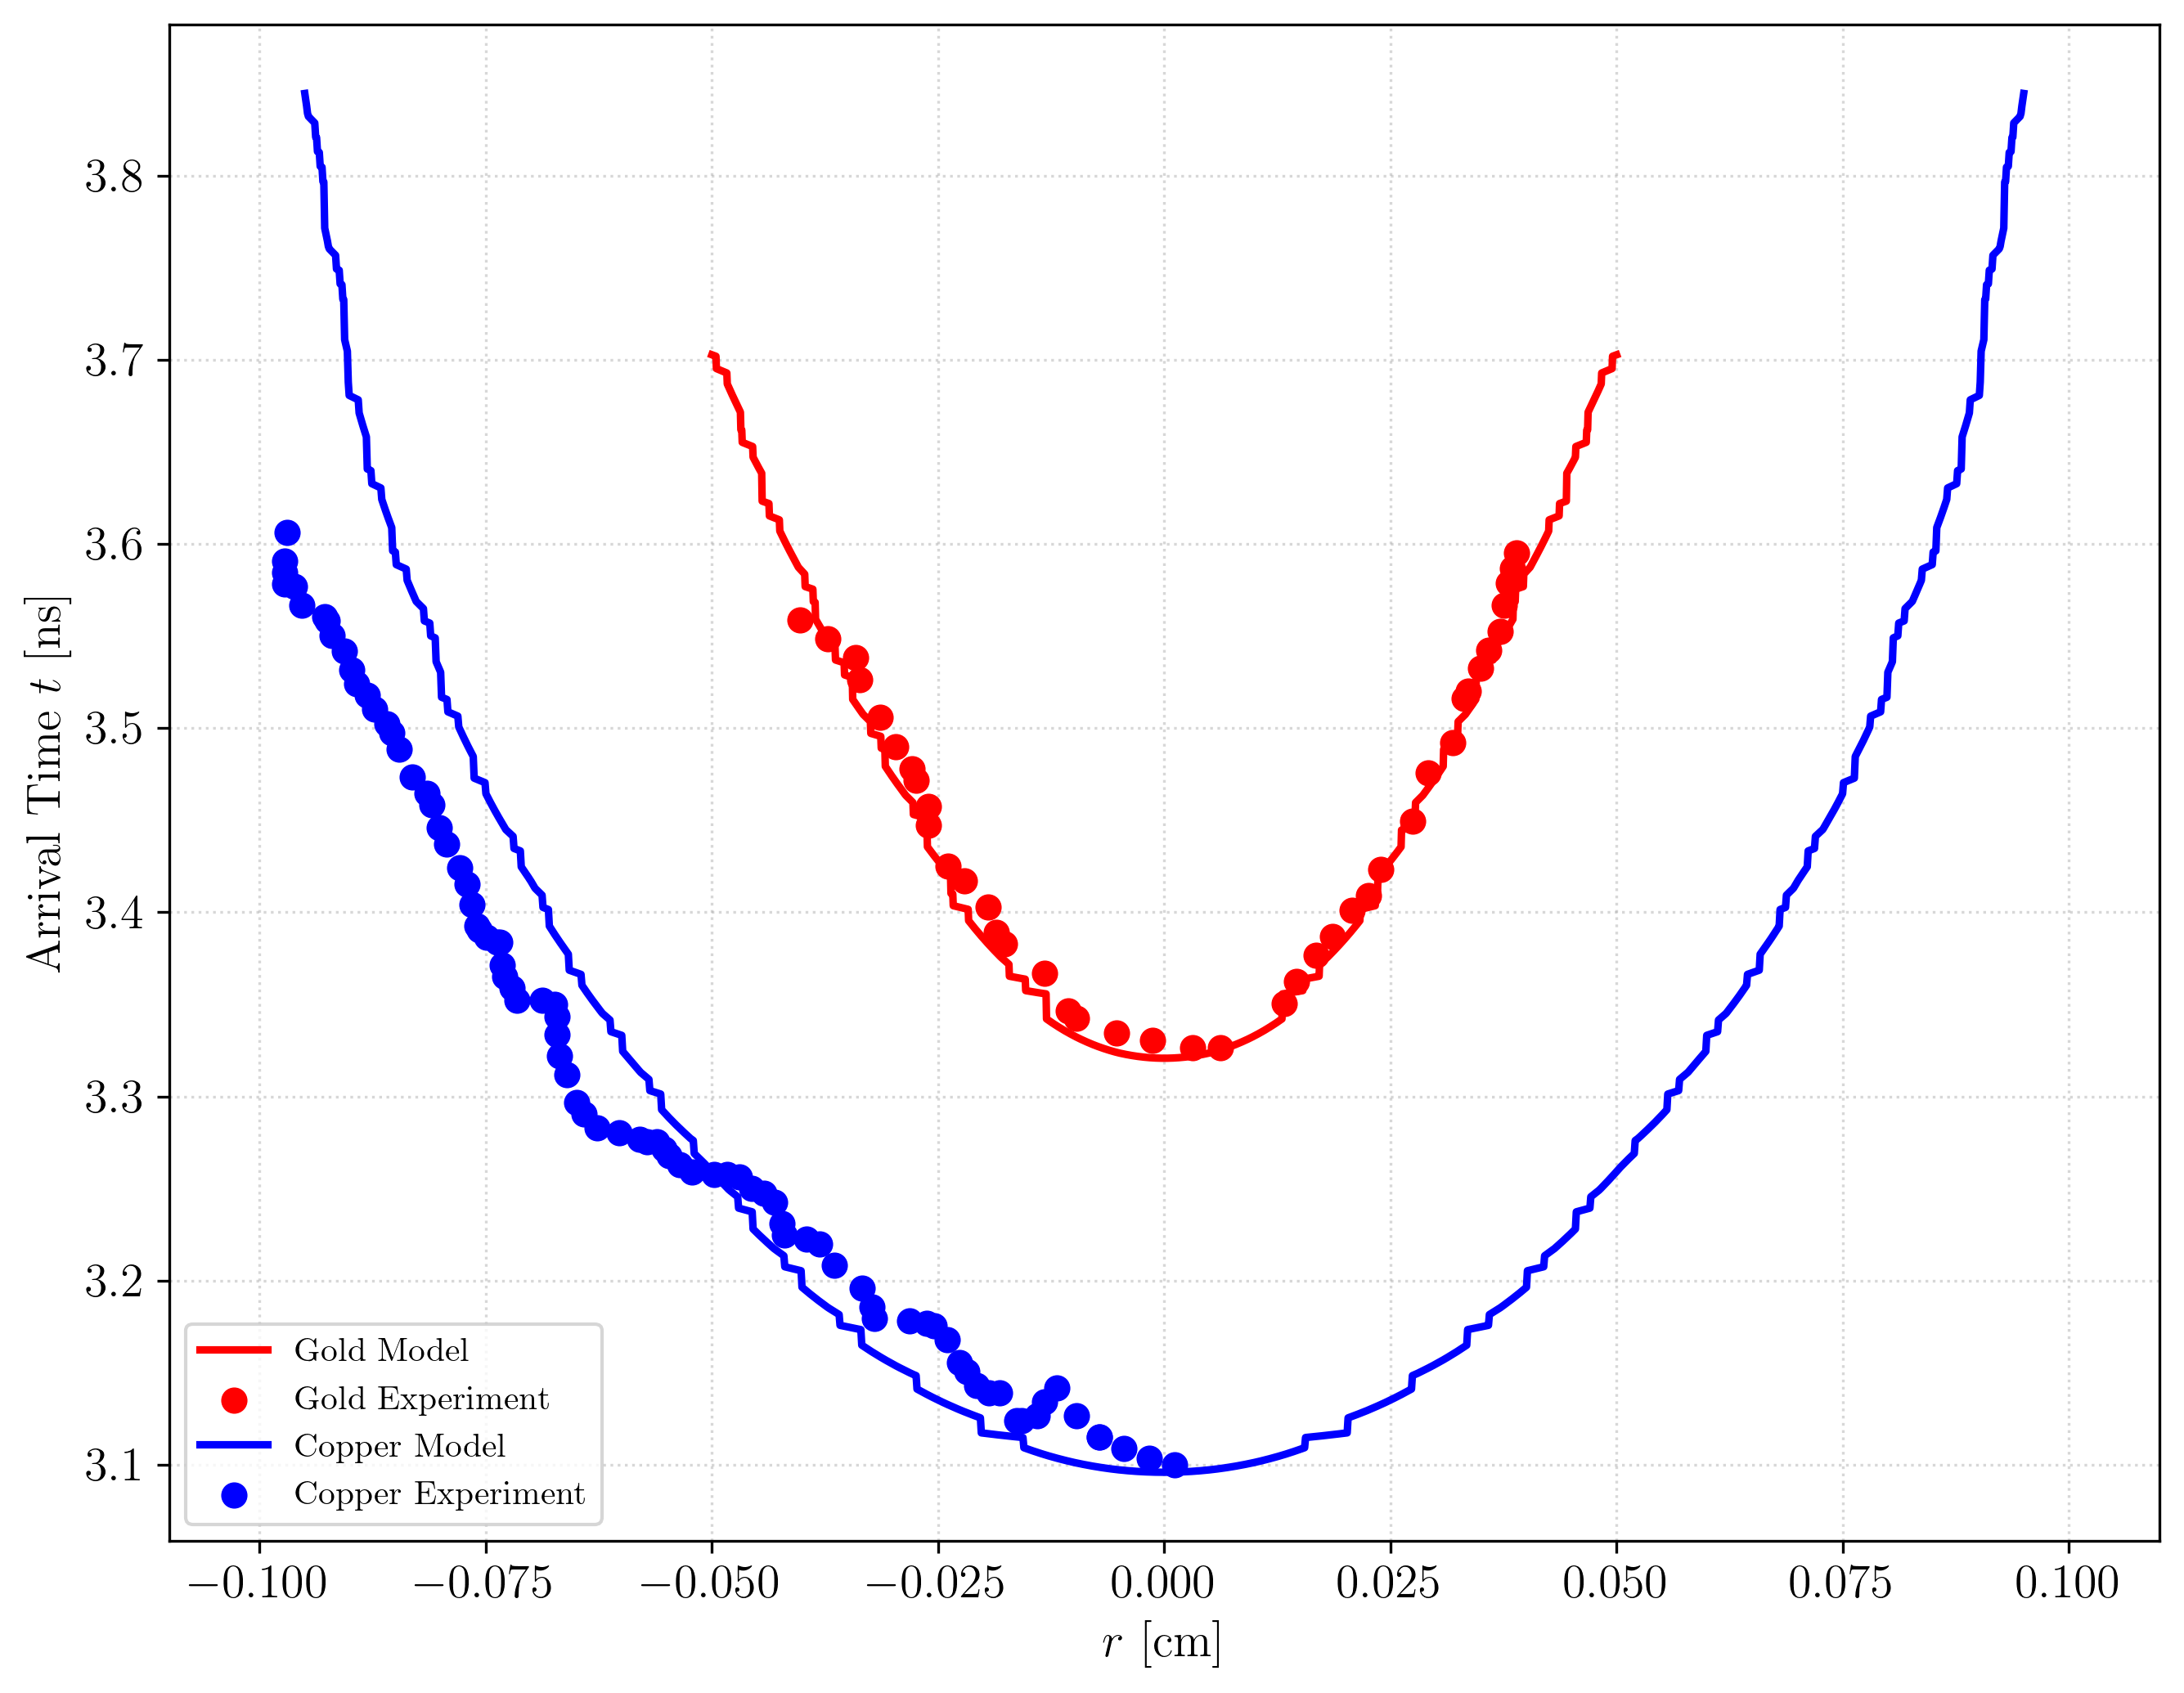
\includegraphics[width=0.75\textwidth]{2D_model/combined_curvature_comparison.png}
    \end{figure}
\end{frame}

% --- Section 4 ---
\section{Conclusion}
\begin{frame}{Conclusion}
    \begin{itemize}
        \item \textbf{Successful 2D Modeling}:
        \begin{itemize}
            \item We have successfully modeled 2D supersonic Marshak waves.
            \item Our unified model captures front curvature and temperature distribution under the diffusion approximation.
        \end{itemize}
        \vspace{0.3cm}
        \item \textbf{Deep Physical Insight}:
        \begin{itemize}
            \item We can now understand the underlying physics of radiation transport and energy exchange in an intuitive and clear manner.
        \end{itemize}
    \end{itemize}
\end{frame}

% put the thank you in a different slide.
{
\setbeamercolor{background canvas}{bg=white}
\begin{frame}[plain]
    \vfill
    \begin{center}
        {\Huge\bfseries\color{black} Thank You!}
        
        \vspace{0.8cm}
        {\LARGE\color{black} Questions?}
    \end{center}
    \vfill
\end{frame}
}

\end{document}